\documentclass{article}

\usepackage{MnSymbol}
\usepackage[backend=biber,style=nature,bibencoding=utf8]{biblatex}
\usepackage{xargs}
\usepackage{listings}
\usepackage{amsfonts}
\usepackage{amsmath}
\usepackage{verbatim}
\usepackage{tikz-uml}
\usepackage{uppaal}
%\usepackage{parskip} % automatically adds line breaks
\usepackage{hyperref}

\usetikzlibrary{arrows}
\usetikzlibrary{arrows.meta}

\tikzset{
vertex/.style={circle,draw,minimum size=1.5em},
edge/.style={->, arrows = {-Latex[length=5pt 3 0]}},
every picture/.style={
        execute at end picture={
                \path (current bounding box.south west) +(0,-0.3) (current bounding box.north east) +(0,0.3);
            }
    }
}

\usepackage{caption}
\captionsetup{font=small, margin=20pt}
\usepackage{subcaption}

\usepackage{graphics}
\usepackage[T1]{fontenc}
\usepackage{multicol}
\usepackage{lipsum}
\usepackage[margin={2cm,2cm}]{geometry}

\addbibresource{bibliography.bib}

\usepackage[capitalise]{cleveref}
\newcounter{defCounter}
\newtheorem{definition}[defCounter]{Definition}
\crefname{defCounter}{Definition}{Definitions}
\crefname{figure}{Figure}{Figures}
\crefname{lstlisting}{Listing}{Listings}

\setlength{\parindent}{0pt}
\usepackage{etoolbox}
\AtBeginEnvironment{definition}{\setlength{\parindent}{-0.45em}}


\newcommand{\semaut}[1]{[\![#1]\!]}
\newcommand{\sembox}[1]{
    #1
}
\newcommandx{\automaton}[7][1=, 2=Q, 3=C, 4=\Delta, 5=\Sigma, 6=s, 7=F]{
    (#2#1, #3#1, #4#1, #5, #6#1, #7#1)
}
\newcommandx{\transition}[6][1=, 2=q, 3=q', 4=\phi, 5=p, 6=a]{
    (#2#1, #4#1, #5#1, #6, #3#1)
}
\newcommandx{\clockreduction}[0]{
    \mathbb{C}_r
}
\newcommandx{\deadedge}[0]{
    \mathbb{T}_d
}
\newcommandx{\deadclock}[0]{
    \mathbb{C}_d
}
\newcommandx{\deadstate}[0]{
    \mathbb{S}_d
}
\newcommandx{\unreachable}[0]{
    \mathbb{S}_u
}
\newcommandx{\pruning}[0]{
    \mathbb{P}
}

\begin{document}

\section*{Summary}
\thispagestyle{empty}

Timed Automata (TAs) are commonly used to verify correct behaviour in real-time systems. Examples could include, finding vital issues in airplane instrumentation, long delays in radio transcriptions and detecting attacks on server infrastructure. Constructing TAs for these use cases, can be enhanced by using Timed Regular Expressions (TREs).

This paper describes the research process, as well as the implementation and functionality of the software product named "Timed Regular Expression to Automaton Transformation" (abbreviated to TREAT).
The program seeks to streamline the use of TREs, as well as serve as a tool for visualizing TREs as TAs.

An existing software product called ``MONAA'' is used for timed pattern matching on timed words. In this regard, it accomplishes a similar goal to this paper, in so far as matching timed words to TREs, though MONAA functions somewhat differently in its use.

The semantic rules that define how TREs are transformed into TAs, are borrowed from the paper "Timed Regular Expressions" by Eugene Asarin et al. Some modifications have been made in order to optimize the generation process, and to fix an error with the semantic rules for creating unions. These semantic rules can create clocks, states, and transitions, that have no effect on the language recognized by the TA. To increase readability, the TAs go through several pruning steps, all of which can be individually disabled by a user of TREAT.
These pruning steps lead to a more minimal TA in terms of number of clocks, states, and transitions, though further improvements could be made, as described in the discussion section.

To further increase readability, this paper describes the implementation of part of the Sugiyama framework, also known as layered graph drawing. This leads to a TA where each state is placed in layers based on the length of the longest path from the initial state. These states are then ordered in each layer, to minimize transition crossings. Our use of this framework leaves some room for improvements, such as fanning out transitions that have the same source and target states, which makes them easier to differentiate.

When performing timed pattern matching over timed words, TREAT requires the assistance of the tool UPPAAL. UPPAAL allows visualization and simulation of TAs.
TREAT is able to output to the XML file format, which can be loaded into UPPAAL. The XML file declares all the information contained in the automaton, as well as any declarations such as variables and clocks. When implementing TREAT, we encountered a number of hurdles, forcing us to find workarounds. An example of this, is the fact that UPPAAL uses int16 as the native integer size, and has no int32 equivalent by default.

As mentioned, TREAT can output in XML format, which can be opened in UPPAAL. This allows the user to verify timed words against the constructed TA. Alternatively, TREAT can also output to a TikZ format, allowing the TA to be used in LaTeX documents.

TREAT sets out to allow users to convert TREs into readable TAs, as well as output those TAs to an external tool (UPPAAL) in order to check a timed word loaded from a .CSV file.
An example usecase is provided in the paper, in which a transcript from the Apollo 11 mission has been converted to a timed word, and a TRE is used as an input for TREAT, which outputs a TA to UPPAAL that can be used to verify the TRE. This example illustrates how TREAT can be utilized on large datasets, with a given TRE, in order to easily perform data analysis.

Finally, we have benchmarked our solution to figure out the best way to prune states while negatively impacting performance as little as possible. These benchmarks showed significant improvements in UPPAAL when using pruning. The benchmarks showed us that pruning can improve performance, whereas the naive pruning (Pruning everything after generation, once) might hinder performance.

We believe that this paper, as well as the TREAT program with its features such as pruning, graph layout, etc., are valuable contributions to the field of Timed Pattern Matching.

\clearpage
\setcounter{page}{1}

\title{Timed Regular Expression to Automaton Transformation}

% \author{
%     Emil Moesby Thomsen\\
%     \small{Dept. of Computer Science}\\
%     \small{Aalborg University}\\
%     \small{etho21@student.aau.dk}
%     \and
%     Frederik Juhl Andreasen\\
%     \small{Dept. of Computer Science}\\
%     \small{Aalborg University}\\
%     \small{fjan21@student.aau.dk}
%     \and
%     Marcus Andersen Lau\\
%     \small{Dept. of Computer Science}\\
%     \small{Aalborg University}\\
%     \small{marla21@student.aau.dk}
% }

\author{Emil Moesby Thomsen$^1$, Frederik Juhl Andreasen$^2$, Marcus Andersen Lau$^3$\\
    \small{Department of Computer Science, Aalborg University}\\
    \small{$^1$etho21@student.aau.dk, $^2$fjan21@student.aau.dk, $^3$marla21@student.aau.dk}}
\maketitle


\begin{multicols}{2}
    \raggedcolumns
    \begin{abstract}
        \textbf{Timed Automata (TAs) are commonly used to verify correct behaviour in real-time systems. Examples could include, finding vital issues in airplane instrumentation, long delays in radio transcriptions and detecting attacks on server infrastructure. Constructing TAs for these use cases, can be enhanced by using Timed Regular Expressions (TREs).}

\textbf{The goal of this paper is to construct Timed Automata from Timed Regular Expressions while optimizing both performance and readability. This is done by defining a number of pruning steps, which eliminate redundant elements in the generated Timed Automata. Along with pruning, implementing an effective layout algorithm further increases visual clarity. The efficiency of this implementation is shown through examples and benchmarks, which also highlight issues, eliciting possible future improvement.}
    \end{abstract}    \section{Introduction}
The formalization of Timed Regular Expressions (TRE) and their equivalence to Timed Automata (TA) was established in the foundational paper ``Timed Regular Expressions'' by Eugene Asarin et al.\cite{Eugene2001}.
This paper demonstrated the construction of TAs from TREs, which is a key focus of this paper.
The ability to convert TREs to TAs allows for modeling of temporal systems.

Tools such as MONAA, MONTRE and UPPAAL have been developed to facilitate analysis and verification of temporal systems.
MONAA performs timed pattern matching on timed words by translating TREs into TAs and can visualize these automata using the DOT language for Graphviz.
UPPAAL, a widely recognized tool in the verification of real-time systems, offers robust functionalities for simulating, visualizing, and verifying TAs.

This paper builds upon the methods described by Asarin et al., focusing on the construction and visualization of TAs from TREs.
We aim to enhance the visual representation of these automata through pruning of unnecessary states, transitions and clocks, as well as the application of the Sugiyama framework, thereby improving their readability.
Pruning states, transitions and clocks also has the advantage of improving performance, both while generating T, and during verification using UPPAAL.
By integrating the capabilities of TikZ and UPPAAL, this paper and the resulting product TREAT (Timed Regular Expression Automata Transformation) contribute to the advancement of the field of Timed Regular Expressions and Timed Automata.
    \section{Related Work}\label{sec:related work}

% TRE paper: https://www-verimag.imag.fr/~maler/Papers/timed.pdf

% structure
%   meta
%   tre paper
%   monaa
%   uppaal
%   graph paper

This section aims to describe and review the literature that has been foundational for the research and work done in this paper. It contextualises the contents and contributions of this paper in the field of Timed Regular Expressions and graph layout visualisations.

The term \textit{timed regular expression} was formalized in the abtly named paper "Timed Regular Expressions" from 2001, written by Eugene Asarin et al.\cite{Eugene2001}. The paper discusses the equivalence between the expressive power of timed automata\cite{ALUR1994} and timed regular expressions. To prove this equivalence, they formalise the construction of timed automata from timed regular expressions, and vice versa. In this paper, only their research on timed regular expressions, and how to construct timed automata from them, is used.

The aforementioned paper on timed regular expressions has been the basis for multiple studies and projects. One such project has resulted in a tool called MONAA. MONAA is a tool used for performing timed pattern matching on timed words \cite{MONAA2017}. When given a timed regular expression, MONAA translates it to an equivalent timed automaton, on which the timed pattern matching is performed. Additionally, since MONAA uses the DOT language for Graphviz \cite{Graphviz} to represent their timed automata, said automaton can be visualized\footnote{MONAAs automata cannot be directly visualised by Graphviz since they use custom attributes, but the developers of MONAA offer a program for converting to automata recognizable by Graphviz\cite{MONAA2017}.}.
% not sure if i should mention that the tregexs used in monaa, are not as powerful as the ones discusses in the paper?

Another aspect of this paper, is finding suitable software for simulating the timed automaton constructed from a given timed regular expression. A tool widely known in the field of verification of real-time systems is UPPAAL. Not only can UPPAAL simulate and visualise timed automata, it can also validate and verify them\cite{UPPAAL}.

UPPAAL represents their systems (collections of timed automata variables etc.) in a handful of formats, the most versatile being XML\cite{UPPAAL}. These XML files contain all the information needed to construct the automata in UPPAAL, including the positions of each individual state. This means that we can use more complex graph layout algorithms to properly visualise timed automata. The paper "Visualisation of state machines using the Sugiyama framework" by Viktor Mazetti et al. describes the theory behind and an implementation of the Sugiyama framework, also known as layered graph drawing, which will be discussed later in this paper \cite{Mazetti2012}.
    \section{Preliminaries}

% THE paper: https://www-verimag.imag.fr/~maler/Papers/timed.pdf

% theory of timed automata: https://www.sciencedirect.com/science/article/pii/0304397594900108


% -Outline automata
% -Explain timed symbols
% -Introduce THE paper


The research in this paper is based on the research done in the paper "Timed Regular Expressions" by Eugene Asarin et al.\cite{Eugene2001}. The Paper describes the equivalence between timed regular expressions and timed automata. Their methods of constructing a timed automaton from a timed regular expression, are used and expanded upon throughout this paper.
An automaton can be defined as a set of states, and a set of transitions between those states. This can be visualized as a directed graph of nodes with edges connecting them.
A timed automaton is a type of automaton that can analyse events happening one after the other, after or within, a specified time, and can be formally defined as a quintuple\cite{ALUR1994}. See \cref{definition:automatonDefinition}.
\begin{definition}\label{definition:automatonDefinition}
    Automaton:
    $$\automaton{}{}{}{}{}{}$$

    $Q$: Finite set of states

    $C$: Finite set of clocks
    
    $\Delta$:Transition relation
    
    $\Sigma$: Alphabet
    
    $s\in Q$:Initial state
    
    $F\subseteq Q$:Accepting states
\end{definition}\cite*{Eugene2001}\\

Clocks are variables that track time. All clocks count up simultaneously, but may be individually reset when a specific transition is taken.

Transition relations are the transitions between states, and may be formally described with the following tuple. See \cref{definition:transition}.

The alphabet is the set of symbols that are accepted by the automaton. The symbols name the events that are to be analysed.

The initial state is the unique state from which the simulation starts, and is entered at time zero.

The accepting states are a set of states that the simulation must be able to reach for a word to be accepted.\\

The words describe sets of events that happen one after the other. A timed automaton is able to analyse timed words, where each event has an associated time, to determine whether the word is accepted by the automaton.

\begin{definition}\label{definition:transition}
    Transition relation:
    $$\Sigma_\epsilon=\Sigma\cup{\epsilon}$$
    $$\Delta\subseteq Q\times\phi\times C\times\Sigma_\epsilon\times Q$$
The tuples have the form $\transition$

$q$: The starting state of the transition

$\phi$: A set of boolean formulas written like $x\in I$

$p$:Clocks to be reset when the transition is taken

$a$: The symbol of the transition

$q'$: The ending state of the transition
\end{definition}\cite*{Eugene2001}

    \section{Implementation}

% input all .tex files from folder
\subsection{Semantics}\label{subsec:semantics}
\begin{comment}
    Where do most of our semantics come from?
    
    Intersection semantics
     - Motivation

    Describe union semantics
     - Motivation
     - New definition
     - Visual change
    
    Describe MatchAny semantics
     - Motivation
     - Definition
     - Visual
\end{comment}

Most of the semantics have been copied directly from the paper by Eugene et al. \cite{Eugene2001}. However we have made a few modifications.

\subsubsection{Intersection}
When creating automata using an intersection with the rules from Eugene et al.
many states are created with no transitions.
By creating the intersection states lazily as needed for transitions, we can greatly decrease the number of states created.
% TODO: Possibly insert a figure here.

\subsubsection{Union}
The only semantics changed from the paper by Eugene et al. is the semantics for union. We noticed the epsilon transitions from the union semantics could be slightly optimized, by only creating an extra epsilon transition when there is a loop going back to the initial state. An updated version of the union semantics can be seen in \cref{def:union-semantics}.

% We can improve upon union by removing unnecessary epsilon transitions.
\begin{definition}
    Union\label{def:union-semantics}
    
    \sembox{
        $\semaut{\varphi_1|\varphi_2}=
        \left\{\begin{array}{ll}
            \semaut{(\epsilon\cdot\varphi_1)\cup\varphi_2} & if (q_1,\phi_1,p_1,a,s_1)\in\Delta_1 \\
            \semaut{\varphi_1\cup(\epsilon\cdot\varphi_2)} & if (q_2,\phi_2,p_2,a,s_2)\in\Delta_2 \\
            \automaton & otherwise \\
        \end{array}\right.
        $
        
        Where
        
        $f\transition=
        \left\{\begin{array}{ll}
            \transition[][s] & if q\in\{s_1,s_2\} \\
            \transition & otherwise \\
        \end{array}\right.
        $
        
        $Q=Q_1\cup Q_2 \cup {s}\backslash\{s_1,s_2\}$
        
        $C=C_1\cup C_2$
        
        $\Delta=f(\Delta_1\cup\Delta_2)$
        
        $F=F_1\cup F_2\backslash\{s_1,s_2\}$
    }
\end{definition}

The semantics work by checking if there is a transition looping back to the initial state on either automaton. If this is the case they are concatenated with an epsilon automaton. That means in the case where both automata have a transition to their initial state, our new semantics will create the same result as the one in the paper. However, when an automaton does not have a transition back to the initial location, we do not need the extra epsilon transition, as the purpose of the extra transition is to make sure you can not first take a loop in one automaton, and then move to the other automaton.

% We can improve upon union by removing unnecessary epsilon transitions.
\begin{definition}
    Union\label{def:union-semantics}
    
    \sembox{
        $\semaut{\varphi_1|\varphi_2}=
        \left\{\begin{array}{ll}
            \semaut{(\epsilon\cdot\varphi_1)\cup\varphi_2} & if (q_1,\phi_1,p_1,a,s_1)\in\Delta_1 \\
            \semaut{\varphi_1\cup(\epsilon\cdot\varphi_2)} & if (q_2,\phi_2,p_2,a,s_2)\in\Delta_2 \\
            \automaton & otherwise \\
        \end{array}\right.
        $
        
        Where
        
        $f\transition=
        \left\{\begin{array}{ll}
            \transition[][s] & if q\in\{s_1,s_2\} \\
            \transition & otherwise \\
        \end{array}\right.
        $
        
        $Q=Q_1\cup Q_2 \cup {s}\backslash\{s_1,s_2\}$
        
        $C=C_1\cup C_2$
        
        $\Delta=f(\Delta_1\cup\Delta_2)$
        
        $F=F_1\cup F_2\backslash\{s_1,s_2\}$
    }
\end{definition}

\subsubsection{Match any}
Only match on a single character was defined in the paper by Euegene et al. and we wanted to have a way to match all possible characters like normal regular expressions and Monaa. For this we used a '.' like in normal regular expressions. Transitions with this symbol are allowed to be taken like any other transition when any input is given. Otherwise this symbol is the same as all other symbols in the automaton.

\usetikzlibrary {automata,positioning}
\begin{tikzpicture}[auto]
    \node[state, initial] at (0, 0)(q0){$q0$};
    \node[state, accepting] at (2, 0)(q1){$q1$};
    
    \path[->]
        (q0)edge node{$.$}(q1)
        ;
\end{tikzpicture}


\subsection{Pruning}\label{sec:pruning}

Some of the semantics from \cref{subsec:semantics} can lead to TA of an explosive size.
An optional pruning step is performed on the automaton, in order to remove transitions, states,
and clocks, that do not affect the transition system.
This leads to better performance (see \cref{subsec:benchmarks}), and better readability. 
%TODO: Affirm claims made about performance after benchmarks

Throughout this section the TA seen on \cref{fig:prune0} will be used as an example of how the prunings work.
The TA is equivalent to the TReg $A_{[1;10]}+'$

% Generated by: TimedRegex, Version = 1.0.0.0
% Date 5/14/2024 6:44:16 PM
\usetikzlibrary {automata,positioning}
\scalebox{0.9}{
    % "C(A[5;10]&(BA|A)[1;3])"
    \begin{tikzpicture}[auto]
        \node[state, initial] at (0, 0)(q0){$q0$};
        \node[state] at (2, 0)(q3){$q3$};
        \node[state] at (2, 4)(q4){$q4$};
        \node[state] at (6, 4)(q7){$q7$};
        \node[state, accepting] at (6, 0)(q2){$q2$};
        
        \path[->]
            (q4)edge node[below]{$A\mid c_1\in[1;3]$}(q7)
            (q3)edge node[above]{$A\mid c_1\in[1;3]$}(q7)
            (q4)edge node[below]{$A\mid c_0\in[5;10]\wedge c_1\in[1;3]$}(q2)
            (q3)edge node[above]{$A\mid c_0\in[5;10]\wedge c_1\in[1;3]$}(q2)
            (q0)edge node[below]{$C\mid <c_0>\wedge<c_1>=0$}(q3)
            ;
    \end{tikzpicture}
}

\captionof{figure}{Lightly pruned automaton, to be used as an example.}
\label{fig:prune0}


\subsubsection{Dead Edge Pruning}\label[subsubsection]{deadEdgePruning}
Edges that are overconstrained on one or more clocks, are considered "dead" edges, and can be removed without changing the language of the automaton.
Since these edges could never be taken by any transition system, it does not change the language to remove them.
Dead edge pruning is formally defined in \cref{definition:deadEdgePruning}.

Pruning dead edges means pruning all edges that can never be taken because they are overconstrained.

We do this by first taking the intersection of all edges with multiple ranges.
If this intersection has no possible values we know the edge cannot possibly be taken.
Since it cannot be taken we can remove it.

Mathematically this can be described as a function ($\mathbb{E}$) taking in an automaton and returning a new automaton with the dead edges being pruned.

\sembox{
    $\deadedge(A)=\automaton[][Q][C][\Delta'][\Sigma][s][F]$
 
    $\Delta'=\{\transition\in\Delta\mid\phi\neq\emptyset\wedge\emptyset\neq\cap_{i=1}^n\phi_i\}$

}

\subsubsection{Unreachable State Pruning}\label[subsubsection]{unreachableStatePruning}
States that are not the destination of any transition or the initial state, are considered "unreachable" states, and can be removed without changing the language of the automaton.
When this rule is applied until continuously, it removes any part of the automaton that is unreachable from the initial state of the TA.
Since these states could never be reached, they were not part of the transition system for any words recognized by the automaton, hence it does not change the language to remove them.
Unreachable state pruning is formally defined in \cref{definition:unreachableStatePruning}

Unreachable states are very similar to dead states.
Except we check for any edges that end at a given state.
If a state is not reachable it is removed.
Repeat until no such states exist.

\sembox{
    $\unreachable(A_1)=\left\{\begin{array}{ll}
        A_1 & if \forall q_1\in Q_1:q_1'\notin F_1\wedge\transition[_1]\in\Delta_1 \\
        \unreachable(\automaton[][Q][C_1][\Delta][\Sigma_1][s_1][F_1]) & otherwise \\
    \end{array}\right.
    $

    $Q=\{q_1'\in Q_1\mid q_1\notin F_1\wedge\transition[_1]\in\Delta_1\}$

    $\Delta=\{\transition[_1]\in\Delta_1\mid q_1'\in Q\}$
}

\subsubsection{Dead State Pruning}\label[subsubsection]{deadStatePruning}
States that are not final states, or the source of any transition,
are considered "dead" states, and can be removed without changing the language of the automaton.
This rule, when applied recursively, effectively removes any branches of the automaton, that do not end in a final state.
Since these states can not reach final states, they were not part of the transition system for any words recognized by the automaton, hence it does not change the language to remove them.
Dead state pruning is formally defined in \cref{definition:deadStatePruning}.

Dead states are all the states that have no way of reaching the final state.
These states are pruned by removing all states that have no edges away from them unless they are final states, this is repeated untill no states satisfy this property.

\sembox{
    $\deadstate(A_1)=\left\{\begin{array}{ll}
        A_1 & if \forall q_1\in Q_1:q_1\notin F_1 \transition[_1]\in\Delta_1 \\
        \deadstate(\automaton[][Q][C_1][\Delta][\Sigma_1][s_1][F_1]) & otherwise \\
    \end{array}\right.
    $

    $Q=\{q_1\in Q_1|q_1\notin F_1\wedge\transition[_1]\in\Delta_1\}$

    $\Delta=\{\transition[_1]\in\Delta_1|q_1\in Q\}$
}

\subsubsection{Dead Clock Pruning}\label[subsubsection]{deadClockPruning}
Clocks that are never used in ranges to constrain any edges are considered "dead", and can be removed without changing the language of the automaton.
Since these clocks never constrain any transitions, it does not change the possible ways to reach final states, hence it does not change the language to remove them.
This rule is formally defined in \cref{definition:deadClockPruning}

% Any clocks that are not used in any intervals can be removed.
% This means removing them both from the clocks set and from any clock resets.
% This shouldn't have a huge impact, but it will allow us to create a more minimal declaration field in Uppaal.
\begin{definition}\label{definition:deadClockPruning}
    Dead clock pruning:
    \vspace{0.5em}

    \sembox{
        $\deadclock\automaton=\automaton[][Q][C'][\Delta'][\Sigma][s][F]$

        \vspace{0.5em}

        $C'=\{c\mid\exists\transition[]\in\Delta:\exists(c',I) \in\phi:c=c'\}$

        $\Delta'=\{\transition[][q][q'][\phi][p\cap C']\mid\transition\in\Delta\}$
    }
\end{definition}
\subsection{Graph Layout}

% Motivation for implementing algorithm ourselves
%   - alternative: use DOT language for Graphviz. 
%       - too much bloat and better understanding of algorithm if implemented manually
% Sugiyama framework
%   - 4 steps
%       - make graph acyclic
%           - mention trivial solution?
%       - assign states to layers
%       - order states in layers
%       - assign positions


% (CDE|(BC)+)|A works well in step 1 and 3, but it does not change from 2 to 3. I can use the reverse tregex in step 2: A|((BC)+|CDE)

% automaton is also missing dummy states

As mentioned in \cref{sec:related work}, the layout algorithm used in (TODO: Insert name of program) to organize and arrange the states in TAs (Timed Automaton), is called the Sugiyama framework, also known as layered graph drawing (TODO: cite sugiyama when \#343 merged). The method comprises four steps that, when combined, results in a layered graph with minimized transition crossings. These steps are discussed below, using the TA shown on \cref{fig:graph_step0}, which was constructed using the following TRE(Timed Regular Expression): $$"(CDE\mid(BC)+)\mid A"$$

% Visualise steps with different automata
\usetikzlibrary {automata,positioning}
\scalebox{0.9}{
    \begin{tikzpicture}[auto]
        \node[state, accepting] at (4, 1)(q0){$q0$};
        \node[state] at (8, 2)(q1){$q1$};
        \node[state] at (3, 3)(q2){$q2$};
        \node[state, accepting] at (2, 2)(q3){$q3$};
        \node[state] at (6, 4)(q4){$q4$};
        \node[state] at (1, 0)(q5){$q5$};
        \node[state, accepting] at (0, 3)(q6){$q6$};
        \node[state, initial] at (6, 0)(q7){$q7$};

        \path[->]
        (q2)edge node{$C$}(q3)
        (q1)edge [bend left=15] node{$B$}(q2)
        (q2)edge [bend left=15] node{$C$}(q1)
        (q5)edge node{$E$}(q6)
        (q4)edge node{$D$}(q5)
        (q7)edge node{$A$}(q0)
        (q7)edge node{$\epsilon\mid c_0\in[0;0]$}(q1)
        (q7)edge node{$C$}(q4)
        ;
    \end{tikzpicture}
}

\subsubsection{Make automata acyclic}
The first step of the Sugiyama framework is to, temporarily, make the automaton acyclic. This is necessary because subsequent steps require transitions to have a consistent direction. As described by Mazetti et al., this is done by reversing a specific list of transitions \cite{Mazetti2012}.
Mazetti describes several methods for finding this list of transitions, including using a depth first search to visit all states, and any transitions that lead to already visited states, should be reversed.
This is the method used by Graphviz' implementation of the Sugiyama framework \cite{Graphviz}. % could be irrelevant

This step, however, is trivially completed during the conversion from a TRE to a TA, since we can deduce where they are by using the semantics described by Eugene et al.
More specifically, in the construction of guaranteed iterator automata, and it's absorbed variant\cite{Eugene2001}.
In the implementation, reversible transitions are completely omitted. This is done because some reversible transitions are self-looping which do not change when reversed $(ex. q9\rightarrow q9)$, and handling all reversible transitions equally makes the algorithm much simpler. This could, however, introduce unforeseen transition crossings when reintroducing the reversible transitions, but we chose the simpler algorithm. A reversible transition can be seen on \cref{fig:graph_step1} (dashed line), described as $q2\rightarrow q1$.
% mention self loops

% insert image of step
\usetikzlibrary {automata,positioning}
\scalebox{0.9}{
    \begin{tikzpicture}[auto]
        \node[state, accepting] at (4, 1)(q0){$q0$};
        \node[state] at (8, 2)(q1){$q1$};
        \node[state] at (3, 3)(q2){$q2$};
        \node[state, accepting] at (2, 2)(q3){$q3$};
        \node[state] at (6, 4)(q4){$q4$};
        \node[state] at (1, 0)(q5){$q5$};
        \node[state, accepting] at (0, 3)(q6){$q6$};
        \node[state, initial] at (6, 0)(q7){$q7$};

        \path[->]
        (q2)edge node{$C$}(q3)
        (q1)edge [bend left=15] node{$B$}(q2)
        (q2)edge [dashed, bend left=15] node{$C$}(q1)
        (q5)edge node{$E$}(q6)
        (q4)edge node{$D$}(q5)
        (q7)edge node{$A$}(q0)
        (q7)edge node{$\epsilon\mid c_0\in[0;0]$}(q1)
        (q7)edge node{$C$}(q4)
        ;
    \end{tikzpicture}
}
\captionof{figure}{Reversible edges omitted (dashed line).}
\label{fig:graph_step1}


\subsubsection{Assign states to layers}
The next step is to assign states to layers. Mazetti et al. describes this process by assigning a given state to the layer index equal to the longest path from the initial state. If a transition spans multiple layers, dummy states are placed to ensure that transitions only move between adjacent layers. \cite{Mazetti2012}

This has been implemented by assigning the initial state of the automaton to layer 0, and assigning the states connected by outgoing transitions to layer 1.
This is done recursively for all outgoing states until a final state is reached.
If, at any point, a state is reached that is on the same layer or lower, it is moved to the next layer, and its outgoing states are recursively updated as well.
Dummy states are introduced if two connected states are more than one layer apart.

This implementation can be seen on \cref{fig:graph_step2}, which has resulted in a much more structured TA.

% insert image of step
\usetikzlibrary {automata,positioning}
\scalebox{0.9}{
    \begin{tikzpicture}[auto]
        \node[state, accepting] at (2, 0)(q0){$q0$};
        \node[state] at (2, -2)(q1){$q1$};
        \node[state] at (5, -2)(q2){$q2$};
        \node[state, accepting] at (7, -2)(q3){$q3$};
        \node[state] at (2, -4)(q4){$q4$};
        \node[state] at (5, 0)(q5){$q5$};
        \node[state, accepting] at (7, 0)(q6){$q6$};
        \node[state, initial] at (0, 0)(q7){$q7$};

        \path[->]
        (q2)edge node{$C$}(q3)
        (q1)edge [bend left=15] node{$B$}(q2)
        (q2)edge [dashed, bend left=15] node{$C$}(q1)
        (q5)edge node{$E$}(q6)
        (q4)edge node{$D$}(q5)
        (q7)edge node{$A$}(q0)
        (q7)edge node{$\epsilon\mid c_0\in[0;0]$}(q1)
        (q7)edge node{$C$}(q4)
        ;
    \end{tikzpicture}
}
\captionof{figure}{States assigned to layers.}
\label{fig:graph_step2}

\subsubsection{Order states in layers}
After all states have been assigned to a layer, they are ordered in those layers to ensure the smallest number of transition crossings. These crossings, more often than not, degrade the visual clarity of the automata.
Mazetti et al. formulates this by sweeping through each layer and ordering its states by the barycenter (average) of the positions of its connected states in the previous layer.
E.g. if a state is connected to two states in the previous layer, and their positions are (0, 0) and (0, 100), the given state's position would be (100, 50).
This sweep is performed thrice, once forward, once backwards, and lastly, forward again.
This ensures that both a given state's incoming and outgoing states play a role in minimizing transition crossings. \cite{Mazetti2012}

The approach implemented for this paper shares the same philosophies as the step described above, and can be seen on \cref{fig:graph_step3}.

% insert image of step
\usetikzlibrary {automata,positioning}
\scalebox{0.9}{
    \begin{tikzpicture}[auto]
        \node[state] at (2, 0)(q0){$q0$};
        \node[state] at (5, 0)(q1){$q1$};
        \node[state, accepting] at (7, 0)(q2){$q2$};
        \node[state] at (2, -2)(q3){$q3$};
        \node[state] at (5, -2)(q4){$q4$};
        \node[state, accepting] at (7, -2)(q5){$q5$};
        \node[state, accepting] at (2, -4)(q6){$q6$};
        \node[state, initial] at (0, 0)(q7){$q7$};

        \path[->]
        (q1)edge node{$E$}(q2)
        (q0)edge node{$D$}(q1)
        (q4)edge node{$C$}(q5)
        (q3)edge [bend left=15] node{$B$}(q4)
        (q3)edge [bend right=15] node{$C$}(q4)
        (q7)edge node{$C$}(q0)
        (q7)edge node{$\epsilon\mid c_0\in[0;0]$}(q3)
        (q7)edge node{$A$}(q6)
        ;
    \end{tikzpicture}
}



\subsubsection{Assign positions}
The last step is to assign positions to each state.
Mazetti et al.'s procedure for this step is to prioritze all states in each layer based on the number of connected states in the previous layer.
More connections give a higher priority. This is quite similar to the previous step except, dummy states are given the highest prioritization.
Each state is placed based on their priority, with the ability to move states with lower priority.
Lastly, transitions between dummy states are merged, and restoring the correct transition oritentations that were reversed in the first step. \cite{Mazetti2012}

As of writing this paper, this approach for assigning positions has not yet been implemented. Instead, states are simply placed based on their layer, and their index on said layer, which already offers much visual clarity. The cycles are reintroduced at the very end of this step. This is reflected in the TA on \cref{fig:graph_step4}.

% insert image of step
\usetikzlibrary {automata,positioning}
\scalebox{0.9}{
    \begin{tikzpicture}[auto]
        \node[state] at (2, 0)(q0){$q0$};
        \node[state] at (5, 0)(q1){$q1$};
        \node[state, accepting] at (7, 0)(q2){$q2$};
        \node[state] at (2, -2)(q3){$q3$};
        \node[state] at (5, -2)(q4){$q4$};
        \node[state, accepting] at (7, -2)(q5){$q5$};
        \node[state, accepting] at (2, -4)(q6){$q6$};
        \node[state, initial] at (0, 0)(q7){$q7$};

        \path[->]
        (q1)edge node{$E$}(q2)
        (q0)edge node{$D$}(q1)
        (q4)edge node{$C$}(q5)
        (q3)edge [bend left=15] node{$B$}(q4)
        (q4)edge [bend left=15] node{$C$}(q3)
        (q7)edge node{$C$}(q0)
        (q7)edge node{$\epsilon\mid c_0\in[0;0]$}(q3)
        (q7)edge node{$A$}(q6)
        ;
    \end{tikzpicture}
}



\subsection{Output Formats}\label[subsection]{output formats}

In order to represent the automaton created from timed regular expressions, 
the intermediate automaton, represented as a C\# class in code, can be output to various formats. 
At the timed of release of this paper, two output formats are supported.

\subsubsection{UPPAAL}
UPPAAL is a state of the art program for representing timed automata \cite*{UPPAAL}. 
When outputting to this format, it is possible to check timed works on the timed regular expression.
This is made possible by the automata created using the timed word, and the declarations in UPPAAL.
Here we define two arrays. One containing the symbols, and one containing the times. 
When all of this is put together, UPPAAL's verifier can check the word by simulating the transition system. 

Outputting to UPPAAL is achieved through translating the automata to an XML file, which can be interpreted by the UPPAAL program.

\subsubsection{TikZ}
TikZ can be used to visualize figures and graphs in LaTeX \cite{Tikz}. TikZ uses some specialized statements for specifying certain parts of a graph.
These statements, as well as common LaTeX statements, are generated from the intermediate automaton, and combined into a LaTeX file.
This output format is useful for getting a simple visualization of one or more automata, as well as dynamically creating visualizations of automata for scientific papers written in LaTeX.

\subsection{Checking}\label{subsec:checking}

% Outputting automata to UPPAAL, allows for checking of timed words, to determine whether they are accepted by the automaton generated from the regular expression. This can be done using UPPAAL's verifier, which simulates the transition system.

% The timed word itself is represented in the declarations section in UPPAAL. In order to check words containing values outside of the bounds of shorts, the type used by the timed word array containing types, uses a custom type that is defined to be of the same size as the integer representing clock values. Here we define two arrays. One containing the symbols, and one containing the times. The alphabet is represented by channels, as well as an automaton with transitions for each symbol, that also increase the index of the timed word arrays. During simulations, the clock ticks up until a symbol time is reached. When this happens, the automaton representing the alphabet takes the corresponding transition. This sends a signal though the channel of the same name, which allows a transition to be taken in the automaton representing the timed regular expression. A timed word is considered to be accepted by the timed regular expression, when the automaton representing the timed regular expression is able to reach a final state.

Using the UPPAAL output format, enables the user to make use of UPPAAL's model checking and verification capabilities.
By constructing a TA representing a given timed word, it is possible to verify that a given TRE satisfies the timing constraints of the timed word.
Given a timed word: $$(A, 0), (A, 2), (B, 3), (B, 3), (A, 8), (B, 12)$$
We can use the following TRE to look for the word ABBA in a span of 10 seconds, which it should find starting at index 1. (assuming the timed word is in seconds): $$(ABBA)[0;10]$$
On such a small timed word, and a trivial TRE it is easy to do manually, but with timed words with thousands of timed events, it is useful to have the ability to automate this with UPPAAL.

\subsubsection{Timed Automaton Representation}\label{subsubsec:ta_rep}
In UPPAAL, TAs are represented by a set of states and transitions connecting these states.
Both states and transitions have properties, but only the properties pertaining to transitions are relavant in this paper. Namely, Guards, Synchronizations and Updates, which are explained on UPPAAL's documentation \cite{UPPAAL}.
The TA shown on \cref{fig:ta_rep} is constructed from the TRE described above. For now, disregard the looping transition on the initial state and the endIndex variable on the last transition, as they will be explained in \cref{subsubsec:verifier}.
\begin{center}
    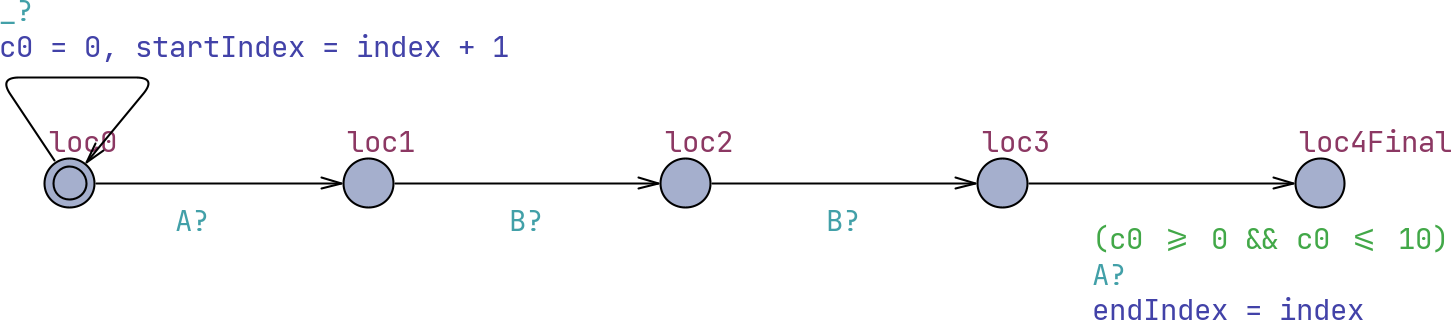
\includegraphics[width=\columnwidth]{Documents/Diagrams/CheckingFigures/checking_tarep.png}
    \captionof{figure}{TA constructed from the TRE $(ABBA)[0;10]$.}
    \label{fig:ta_rep}
\end{center}
The word is recognized by the TA, if the execution terminates at an accepting state.
In the case of the TA on \cref{fig:ta_rep}, the only accepted word is ABBA, and it is only accepted if the 4 symbols appear within 10 seconds of eachother.

The accepting state can only be reached by traversing the graph's transitions, and these transitions have been constructed to meet the requirements of the TRE. Each symbol in the TRE is converted into a datatype called a Broadcast Channel \cite{UPPAAL}. While the documentation says they are used to synchronize processes (TA), the intuition in this paper, is that they are used to send and receive signals across channels. The syntax is as following:
\begin{itemize}
    \setlength\itemsep{-0.5em}
    \item $x!$ - Outgoing signal (send)
    \item $x?$ - Incoming signal (receive)
\end{itemize}
Where $x$ is any symbol. This syntax is used in Synchronizations on transitions. On \cref{fig:ta_rep}, each transition has an incoming synchronization label, meaning that each transition can only be traversed, when the corresponding signal is given. The outgoing signals will be administered by timed words. On the last transition in the TA, an additional Guard label is present, which represents the timing constraint. Along with an incoming signal, the clock $c0$ has to be within 10 seconds for the transition to fire.

\subsubsection{Timed Word Representation}\label{subsubsec:tw_rep}
In UPPAAL, timed words are represented by two arrays. One array for the symbols of the timed word, and another for the times. This way, the two arrays form pairs of symbols and their corresponding times. The timed word described above would be written like this:

\begin{lstlisting}[basicstyle=\scriptsize]
    const string word[7] = {"A", "A", "B", "B", 
                            "A", "B", "\0"};
    clock_t times[7] = {0, 2, 3, 3, 8, 12, 13};
\end{lstlisting}
\captionof{lstlisting}{Timed word in UPPAAL.}
\label{lstlisting:timed_word}

From this timed word, a TA can be constructed to interact with the other TA constructed from the TRE. This TA can be seen on \cref{fig:tw_rep}.

\begin{center}
    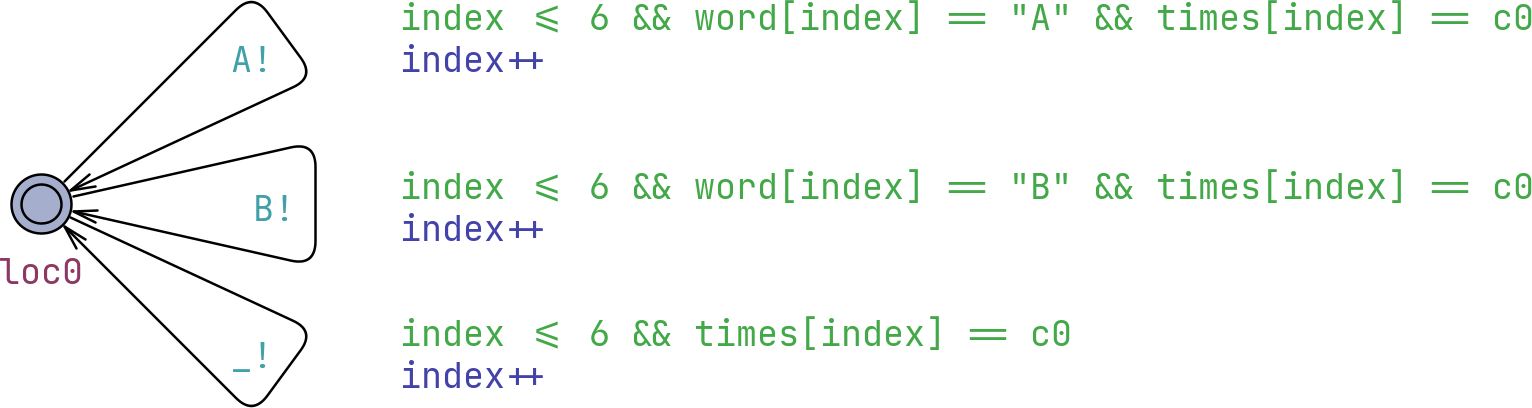
\includegraphics[width=\columnwidth]{Documents/Diagrams/CheckingFigures/checking_twrep.png}
    \captionof{figure}{Timed word TA for \cref{lstlisting:timed_word}. Positions heavily modified for visual clarity.}
    \label{fig:tw_rep}
\end{center}

The TA consists of a single state, and one looping transition for each unique symbol in the timed word, plus an extra transition that matches any symbol.
Each transition has a Guard, a Synchronization and an Update. Take the transition for the symbol $A$.
It boils down to: "\textit{If the current symbol is $A$ and the current time matches its timestamp (Guard), send a signal on channel $A$(Synchronization) and move to the next symbol (Update).}"
This is the case for all transitions, except the match-any transition, since it sends a signal for each symbol in the timed word. The signals sent by the outgoing Synchronizations are ofcourse being received by the TA on \cref{fig:ta_rep}, which potentially progresses the TA. If there is a sequence of symbols in the timed word that matches the initial TRE, the TA should reach the accepting state. UPPAAL has a tool that makes this process of verification much simpler.

\subsubsection{Verifier}\label{subsubsec:verifier}
The verifier in UPPAAL can be used to check a multitude of properties of a given TA, but in this project, it is only used to check if the TA has reached an accepting state. The query on \cref{lstlisting:query} shows the query for checking just that for the TA on \cref{fig:ta_rep}.

\begin{lstlisting}[basicstyle=\scriptsize]
    inf{ta0.startIndex >= 0 && (ta0.loc4Final)} : 
    ta0.startIndex, ta0.endIndex
\end{lstlisting}
\captionof{lstlisting}{Query for checking if accepting state is reached.}
\label{lstlisting:query}

All query syntax and semantics can be found on UPPAAL's documentation \cite{UPPAAL}, but this specific query is structured like this:
\begin{lstlisting}[basicstyle=\scriptsize]
    operation{condition} : subject
\end{lstlisting}
finds the infimum of startIndex and endIndex shown in \cref{fig:ta_rep}, but only if startIndex is initialized and the TA has reached an accepting state. The infimum operation finds the minimum value of the subject given the condition is true, which in this case finds the first occurence of $ABBA$ in the timed word.

When using TREAT, and the output format is UPPAAL (which is default), this query is generated, but cannot be properly utilized without a timed word, which can be specified.

\subsubsection{Shortcomings}\label{subsubsec:shortcomings}
We have encountered some limitations with UPPAAL, that we have had to work around.

% int sizes (shorts (summer))
% vi repræsenterer indices med floats, men uppaal er det int16
% clocks højeste værdi er 2^30-2, hvilket clasher med int16
% clock_t i typedef
% floating point clocks ??

One of the most prominent issues we found is with UPPAAL's integer size, which is equal to a short, only 16 bits. This meant, that when implementing timed words, the elements in the times array had a maximum bound of 32.767, which is fine for smaller timed words, but they can contain millions of timed events. In UPPAAL, it is possible to define custom datatypes, and since we compare these times in the array to clock, in the following example, we thought to define a datatype with the same size as the clock datatype.

\begin{lstlisting} [basicstyle=\scriptsize]
    word[index] == "A" && times[index] == c0
\end{lstlisting}

The UPPAAL documentation does not say much on the clock datatype, however, through trial and error we have found it to be of the size $2^{30}-2$ bits.
This further cements that the integer size is a bottleneck to our implementation, which limits us to a relatively small maximum bound for timed words.
With the actual size of clocks, we defined a new datatype called \verb|clock_t|, which has been used on \cref{lstlisting:timed_word}. It is defined to be the same size as the clock datatype, and declared as follows in the system declaration in UPPAAL:

\begin{lstlisting} [basicstyle=\scriptsize]
    typedef int[-1073741822,1073741822] clock_t;
\end{lstlisting}

This means that TREAT can handle much larger timed words.

% RAM issues (works fine on linux, nono on windows)
% output where match occurs
%   diagnostic trace gives
%   just output start and end indices
\subsection{The Product}\label{subsec:theProduct}
The research in this paper has culminated in a software product that allows a user to enter a timed regular expression (TRE), and have it converted into a timed automaton (TA).
We have named this piece of software "TREAT", short for "Timed Regular Expression to Automaton Transformation".

TREAT is accessed through a command line interface. The user can type in their TRE, along with a few options such as adding a timed word through a .csv file, turning off pruning, and silencing any warnings or info messages.
The user can also decide the output format of the TA at this point, if it has not already been specified. 

If the user opted to add a timed word, it is loaded from the .csv file, into two arrays. Each unique symbol in the word is added to the alphabet.
An automaton is created, that represents the timed word. This is required for checking the TRE with UPPAAL. This automaton has an edge for each of the symbols of the alphabet, and broadcasts its symbol on channels at the correct time. Checking is described further in \cref{subsec:checking}.

The TRE is parsed into tokens by a tokenizer. These tokens are connected as children of one another, to form an abstract syntax tree (AST). 
From the AST, the TA can be created using the rules from Eugene et al., with the modifications described in \cref{subsec:semantics}.

This is done by visiting each node in the tree, and generating states and edges in the TA, according to the rules. Three visitors go through the tree: One checks whether intervals on any given transition are valid. Another goes through the AST, to convert the iterator and the absorbed iterator into lower level components using union and iterator. The last visitor is responsible for implementing the rules of all other tokens.

At this stage, the TA is pruned as described in \cref{subsec:pruning}. 
% The dataformat of the internal TA is an object containing hashsets and dictionaries corresponding to the sets of the tuples described in \cref{sec:preliminaries}. 
% This means that the code executed in the functions responsible for pruning, map very closely to the mathematical operations in \cref{sec:preliminaries}.

Since the TA is now in its final form with regards to states, transitions, and the guards associated with them, each state is now assigned a position based on the algorithm described in \cref{subsec:graph}.

Finally, the TA is output to one of the selected formats as described in \cref{subsec:formats}.





% \subsubsection{Command Line Interface}

% \subsubsection{Tokenizer}

% \subsubsection{AST}

% \subsubsection{Automaton Generator}

% \subsubsection{Pruning}

% \subsubsection{Location Assignment}

% \subsubsection{Output}

% \subsubsection{Timed Words}


    \section{Discussion}

% input all .tex files from folder
\subsection{Readability}

\subsubsection{Graph Layout}
% missing from graph paper
The Sugiyama Layout algorithm discussed in \cref{subsec:graphlayout} served the purpose of increasing visual clarity and readability of the TA outputted by TREAT.
Two of the most prevalent ways this was achieved was by layering the TAs states based on the length of the longest path from the initial state. The other was by ordering the states in each layer to achieve the smallest number of edge crossings.
While some of the specific approaches described by Mazetti et al. \cite{Mazetti2012} was not implemented into TREAT, the resulting implementation still greatly increases readability.

As mentioned in \cref{subsec:graphlayout}, the last step of the Sugiyama framework was not implemented, namely, properly positioning states in relation to each other. This might be developed in the future.

Another feature that would unequivocally improve readability is to visually separate transitions that share states, such as reversible transitions.
In all TAs pictured in \cref{subsec:graphlayout} and this section, any such transitions have been manually separated, since this feature has not been implemented. The difference can be seen on \cref{fig:transitions}.

\begin{center}
    \usetikzlibrary {automata,positioning}
\scalebox{0.9}{
    \begin{tikzpicture}[auto]
        \node[state] at (0, 0)(q0){$q0$};
        \node[state] at (2, 0)(q1){$q1$};
        \node[state] at (5, 0)(q2){$q0$};
        \node[state] at (7, 0)(q3){$q1$};

        \path[->]
        (q0)edge (q1)
        (q1)edge (q0)
        (q2)edge [bend left=15] (q3)
        (q3)edge [bend left=15] (q2)
        ;
    \end{tikzpicture}
}
\vspace{-1em}
\captionof{figure}{Comparison between implementation(Left) and intended behaviour(Right)}
\label{fig:transitions}
\end{center}

% formats
As described in \cref{output formats}, two output formats can be used to represent TAs.
The first format is UPPAAL. In UPPAAL, if no positions are given, the states are simply placed in a grid. This means, that using a graph layout algorithm is not strictly necessary.
To show its advantages, however, \cref{fig:treatLayout} shows the TA described in \cref{subsec:graphlayout}, which uses TREATs positioning, while \cref{fig:uppaalLayout} shows UPPAALs positioning. Both of these figures are constructed in UPPAAL

\begin{center}
    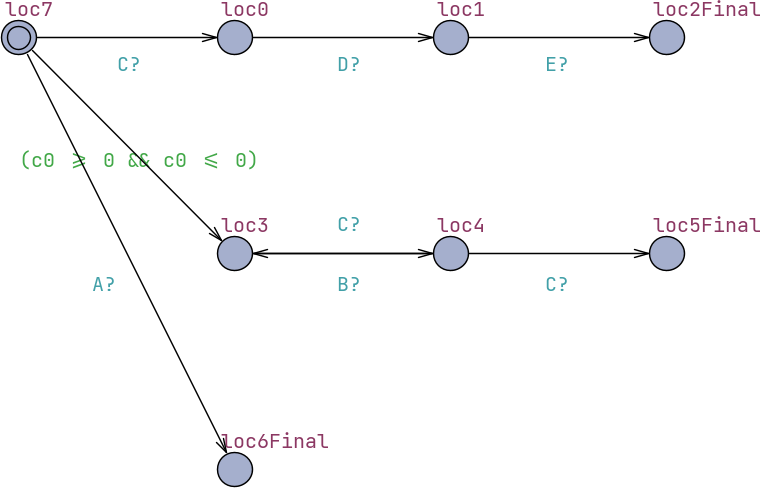
\includegraphics[width=0.8\columnwidth]{Documents/Diagrams/ReadabilityFigures/treat.png}
    \captionof{figure}{TA with TREATs state positioning.}
    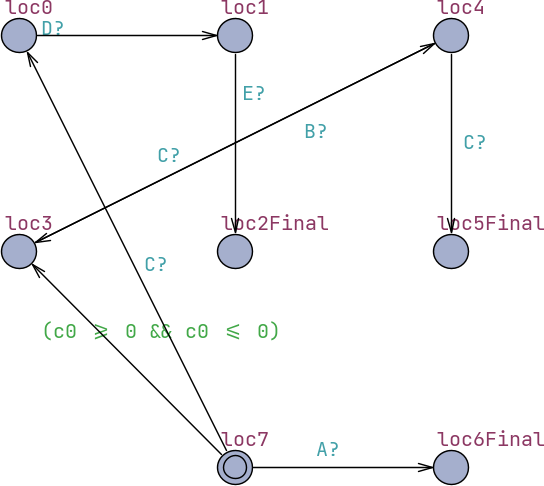
\includegraphics[width=0.6\columnwidth]{Documents/Diagrams/ReadabilityFigures/uppaal.png}
    \captionof{figure}{TA with UPPAALs state positioning.}
\end{center}
\vspace{1em}

The other output format is TikZ, used to represent graphs in LaTeX. Unlike UPPAAL, states in TikZ need positions, which necessitates some form of graph layout algorithm.

\subsubsection{Pruning}

The pruning steps described in \cref{sec:pruning} have an arguably greater effect to readability, since this can dramatically reduce the size and complexity of the output TA, while having no effect on the language accepted by the TA.
The TA on \cref{fig:nopruning} represents the same TRE as the one on \cref{fig:treatLayout}, except, no unreachable states, dead states, or dead transitions have been pruned.

\begin{center}
    \usetikzlibrary {automata,positioning}
% "(CDE|(BC)+)|A"
\begin{tikzpicture}[auto]
    \node[state] at (2, 0)(q0){$q0$};
    \node[state] at (2, -2)(q1){$q1$};
    \node[state] at (4, 0)(q2){$q2$};
    \node[state] at (4, -2)(q3){$q3$};
    \node[state, accepting] at (6, 0)(q4){$q4$};
    \node[state] at (2, -4)(q5){$q5$};
    \node[state] at (4, -6)(q6){$q6$};
    \node[state] at (4, -4)(q7){$q7$};
    \node[state, accepting] at (6, -2)(q8){$q8$};
    \node[state, accepting] at (2, -6)(q9){$q9$};
    \node[state, initial] at (0, 0)(q10){$q10$};

    \path[->]
    (q1)edge node{$D$}(q2)
    (q3)edge node{$E$}(q4)
    (q1)edge node{$D$}(q3)
    (q5)edge node{$B$}(q6)
    (q7)edge node{$C$}(q8)
    (q5)edge [bend left=15] node{$B$}(q7)
    (q7)edge [bend left=15] node{$C$}(q5)
    (q10)edge node{$C$}(q0)
    (q10)edge node{$C$}(q1)
    (q10)edge node{$\epsilon\mid c_0\in[0;0]$}(q5)
    (q10)edge node{$A$}(q9)
    ;
\end{tikzpicture}
\captionof{figure}{Graph layout with all pruning disabled.}
\label{fig:nopruning}
\end{center}
% maybe this figure is too big to include in the paper?

While disabling pruning on this example TA has significantly lowered the visual clarity, the TRE it represents is quite simple, and more complex TREs would only worsen the effect. This shows that pruning is a necessary step to ensure readability and visual clarity.
\subsection{Benchmark UPPAAL}\label{sub:benchmark_uppaal}
More states should intuitively mean UPPAAL runs slower, however this might not be the case if these extra states are easily pruneable.
Therefore we tried running the same query twice in UPPAAL on a large timed word.
The timed word used in these examples are 34198 timed characters long, and the last character happens at time 238817.
The data of these benchmarks can be found on \cref{table:uppaal_benchmarks}.

\begin{tabular}{|c|c|c|c|c|}
    \hline
    & States & Edges & Clocks & Time \\
    \hline
    Pruning & 6 & 8 & 3 & 76s \\
    \hline
    No pruning & 10 & 12 & 3 & 103s \\
    \hline
\end{tabular}
\captionof{table}{Table of benchmarks in UPPAAL.}
\label[table]{table:uppaal_benchmarks}

As can be seen on \cref{table:uppaal_benchmarks}, checking is faster with pruning.
This points to UPPAAL not pruning the unnecessary states when checking.
So pruning not only helps with readability, it also helps with performance. 

\subsection{Benchmark TREAT}
\subsubsection{Setup}
Next step is checking if the prunings have an effect on performance on TREAT.
In the original implementation, all pruning steps were performed after generating the entire automaton.
However, it might be faster if pruning is performed while generating the automaton.
For this reason, we have created a series of TREs and test configurations, and put them all against each other to see how each perform.
Each configuration is a mix of pruning before and after generation of the automaton.

\begin{enumerate}
    \item \textbf{N}: This configuration has no pruning.
    \item \textbf{S}: This configuration prunes only states after generation.
    \item \textbf{E}: This configuration prunes everything after generation.
    \item \textbf{SS}: This configuration prunes states during generation and only states after generation.
    \item \textbf{SE}: This configuration prunes states during generation and everything after generation.
    \item \textbf{ES}: This configuration prunes everything during generation and only states after generation.
    \item \textbf{EE}: This configuration prunes everything during generation and everything after generation.
\end{enumerate}

Note: When we say prune during generation, we are talking about pruning the operands of the explosive operators.
This means the left and right operand of an intersection and the single operand of an absorbed iterator.

As for the tests, we have generated 6 parameterized TREs, that we use to generate a total of 19 unique TREs.
Each TRE serves a unique purpose.
All these TREs can be found in \cref{app:RegularExpressionTable}.

TREs $a$, $b$ and $f$ were all chosen because they would benefit from pruning while generating.
, serving as a best case scenario for SS, SE, ES and EE.
The theory is, that these configurations limit the amount of states used in the explosive operators, therefore making them less explosive.
Ideally it should make them resemble a linear complexity, since the final TAs are of constant length.

TRE $c$, $d$ and $e$ where all chosen to benefit no pruning while generating.
, serving as a best case scenario for N, S and E.
The theory is, these regular expressions will not benefit from pruning while generating, since limited or no pruning can be done during generation.

\subsubsection{Results}
The results can be split into 3 main categories.

\begin{enumerate}
    \item Equivalent performance between configurations.
    \item SS, SE, ES and EE configurations are better.
    \item N, S, SS configurations are better.
\end{enumerate}

All the plots can be seen on \cref{sec:BenchmarkGraphs}, with all the data on \cref{sec:BenchmarkTable}, however a few will be presented here.
On all the graphs we see the relationship between time to run/memory usage (y-axis) and a value for how long the regular expression is (x-axis). The value is explained further in \cref{sec:RegularExpressions}.

The TREs $a$, $b$, $d$ and $e$ are all equivalent in performance.
By this we mean their graphs are all curved in the same way, and they are within a few percentages of each other.
An example of this can be seen on \cref{fig:mean3-5} (this is the one with the biggest difference in this category).

\resizebox{\columnwidth}{!}{
    % 3,4,5
\plot{1,2,4}
{(1,5352.0)(2,33275.6)(4,14345441.6)}
{(1,7892.0)(2,46225.8)(4,21889111.1)}
{(1,6849.0)(2,39386.9)(4,15581794.2)}
{(1,5774.6)(2,18779.8)(4,6445558.3)}
{(1,6492.7)(2,21796.9)(4,9163154.7)}
{(1,6098.4)(2,17999.6)(4,3569375.9)}
{(1,6843.2)(2,20351.3)(4,5761799.7)}
}

\resizebox{\columnwidth}{!}{
    % 3,4,5
\plot{1,2,4}
{(1,5352.0)(2,33275.6)(4,14345441.6)}
{(1,7892.0)(2,46225.8)(4,21889111.1)}
{(1,6849.0)(2,39386.9)(4,15581794.2)}
{(1,5774.6)(2,18779.8)(4,6445558.3)}
{(1,6492.7)(2,21796.9)(4,9163154.7)}
{(1,6098.4)(2,17999.6)(4,3569375.9)}
{(1,6843.2)(2,20351.3)(4,5761799.7)}
}
\captionof{figure}{Graphs for time and memory of regular expression 3-5 ($b$).}
\label{fig:mean3-5}

Since we were expecting $a$ and $b$ to be more performant on SS, SE, ES and EE, this result is not what we expected.
After opening up one of the automata (\cref{fig:FailedPruning}) we can see state $q1$ should have been pruned, since it can never be reached from the initial state.
However, it is not pruned, because it is neither unreachable nor dead because of the self loop.
So we have a problem where a loop to a state itself will keep a state throughout our pruning rules.

% File Generated Automatically
%
% NOTICE: This file has been generated automatically.
% Any manual modifications made to this file may be
% overwritten the next time it is generated.
%
% Generated by: TimedRegex, Version = 1.0.0.0
% Date 5/24/2024 10:27:37 AM
\usetikzlibrary {automata,positioning}
% "((J)+')+'"
\begin{tikzpicture}[auto]
    \node[state, initial] at (6, 0)(q0){$q0$};
    \node[state] at (9, 0)(q1){$q1$};
    \node[state, accepting] at (12, 0)(q2){$q2$};
    \node[state, accepting] at (9, 3)(q3){$q3$};
    
    \path[->]
        (q1)edge node{$J$}(q2)
        (q1)edge node{$J$}(q0)
        (q0)edge node{$J$}(q3)
        (q0)edge [loop above] node{$J$}(q0)
        (q1)edge [loop above] node{$J$}(q1)
        (q0)edge [loop above] node{$J$}(q0)
        ;
\end{tikzpicture}
 

\captionof{figure}{A fully pruned automata with a self loop that could be pruned.}
\label{fig:FailedPruning}

Creating bigger automata only expands on this problem. This is something that could be fixed, but for now we are leaving it as is.

The TRE $f$ performs better on SS, SE, ES and EE.
This graph can be seen on \cref{fig:mean15-19}.
This is the kind of performance difference we expected, and proves pruning during generation is a lot better for intersection.

\resizebox{\columnwidth}{!}{
    % 15,16,17,18,19
\plotmem{1,2,4,8,16}
{(1,2.38) (2,12.3)(4,59.38)(8,917.55)   (16,315469.2)}
{(1,4.75)(2,15.5)(4,83.24)(8,2515.32)  (16,1955655.8)}
{(1,3.73)(2,13.86)(4,62.1)(8,934.43)   (16,321366.52)}
{(1,3.73)(2,13.37)(4,33.36)(8,76.75)    (16,174.71)}
{(1,4.75)(2,14.63)(4,36.13)(8,86.02)    (16,208.98)}
{(1,3.73)(2,15.4)(4,39.59)(8,89.39)    (16,193.98)}
{(1,4.75)(2,16.66)(4,40.86)(8,90.66)    (16,195.24)}
}

\resizebox{\columnwidth}{!}{
    % 15,16,17,18,19
\plotmem{1,2,4,8,16}
{(1,2.38) (2,12.3)(4,59.38)(8,917.55)   (16,315469.2)}
{(1,4.75)(2,15.5)(4,83.24)(8,2515.32)  (16,1955655.8)}
{(1,3.73)(2,13.86)(4,62.1)(8,934.43)   (16,321366.52)}
{(1,3.73)(2,13.37)(4,33.36)(8,76.75)    (16,174.71)}
{(1,4.75)(2,14.63)(4,36.13)(8,86.02)    (16,208.98)}
{(1,3.73)(2,15.4)(4,39.59)(8,89.39)    (16,193.98)}
{(1,4.75)(2,16.66)(4,40.86)(8,90.66)    (16,195.24)}
}
\captionof{figure}{Graphs for time and memory of regular expression 15-19 ($f$).}
\label{fig:mean15-19}

Finally, the TRE $c$ performs better on N, S and SS.
This graph can be seen on \cref{fig:mean6-8}
This is probably because the pruning of everything is too expensive in terms of time and memory for it to make sense for this automaton.
While this is an interesting result, it does not mean these prunings are better, since they do not get rid of all the extra states.

\resizebox{\columnwidth}{!}{
    % 6,7,8
\plotmem{64,128,256}
{(64,2774.94)    (128,9617.03)     (256,36055.38)}
{(64,158752.09)  (128,1245220.51)  (256,9871874.21)}
{(64,2799.35)    (128,9667.24)     (256,36160.29)}
{(64,2338.61)    (128,8618.71)     (256,33125.43)}
{(64,14810.97)   (128,102171.73)  (256,756806.44)}
{(64,112051.15)  (128,884427.52)  (256,7031719.82)}
{(64,124523.45)  (128,977979.83)  (256,7755400.13)}
}

\resizebox{\columnwidth}{!}{
    % 6,7,8
\plotmem{64,128,256}
{(64,2774.94)    (128,9617.03)     (256,36055.38)}
{(64,158752.09)  (128,1245220.51)  (256,9871874.21)}
{(64,2799.35)    (128,9667.24)     (256,36160.29)}
{(64,2338.61)    (128,8618.71)     (256,33125.43)}
{(64,14810.97)   (128,102171.73)  (256,756806.44)}
{(64,112051.15)  (128,884427.52)  (256,7031719.82)}
{(64,124523.45)  (128,977979.83)  (256,7755400.13)}
}
\captionof{figure}{Graphs for time and memory of regular expression 6-8 ($c$).}
\label{fig:mean6-8}

\subsubsection{Conclusions}
We have shown that, in UPPAAL, you can gain significant performance by pruning the states.
, so pruning should be worth it to do most of the time, since pruning is a startup cost.

Pruning by itself can lead to really explosive performance on some regular expressions.
, even if we prune while the automaton is generating.
However, in general, it seems like pruning during generation has the ability to turn some generations from parabolic to linear.

\subsection{Usecases}\label{subsec:usecases}

% apollo 11 transcript, link to it
% do a runthrough of how it could be used to find interesting things

This section will detail and run through a couple of usecase examples, documenting the process of using TREAT from the CLI.

The first example is the most extensively tested usecase, and involves the Apollo 11 Air-To-Ground Voice Transcription (can be found at \url{https://www.nasa.gov/history/alsj/a11/a11transcript_tec.html}). For the purposes of this example, the transcript in its current form is not desirable, so it should be converted into a timed word. \cref{lstlisting:transcript} shows this conversion for the first 62 seconds of the transcription.

\lstdefinestyle{transcript}{
    basicstyle=\scriptsize\ttfamily,
    escapeinside={|*}{*|},
    emphstyle=[2]\textcolor{purple},
    emphstyle=[3]\textcolor{lightgray},
    emph=[2]{LMP, CC, CDR, CMP, CT, MSFN, SC, CDF, MS, PRESIDENT, HORNET, SWIM1},
    emph=[3]{message},
    literate=
        {0}{{\textcolor{teal}0}}{1}%
        {1}{{\textcolor{teal}1}}{1}%
        {2}{{\textcolor{teal}2}}{1}%
        {3}{{\textcolor{teal}3}}{1}%
        {4}{{\textcolor{teal}4}}{1}%
        {5}{{\textcolor{teal}5}}{1}%
        {6}{{\textcolor{teal}6}}{1}%
        {7}{{\textcolor{teal}7}}{1}%
        {8}{{\textcolor{teal}8}}{1}%
        {9}{{\textcolor{teal}9}}{1}%
        {<}{{\textcolor{lightgray}<}}{1}%
        {>}{{\textcolor{lightgray}>}}{1}%
}

\begin{center}
    \captionsetup{width=0.45\columnwidth}
    \begin{minipage}{.6\columnwidth}
        \begin{lstlisting}[style=transcript]
    00 00 00 04 CDR <message>
    00 00 00 13 CDR <message>
    00 00 00 15 CMP <message>
    00 00 00 34 CDR <message>
    00 00 00 44 CDR <message>
    00 00 01 02 CC  <message>
    |*$\vdots$*|
        \end{lstlisting}
    \end{minipage}$\Longrightarrow$
    \begin{minipage}{.25\columnwidth}
        \begin{lstlisting}[style=transcript]
    CDR, 4
    CDR, 13
    CMP, 15
    CDR, 34
    CDR, 44
    CC,  62
    |*$\vdots$*|
        \end{lstlisting}
    \end{minipage}
\end{center}
\vspace{-1em}
\captionof{lstlisting}{Transcript (Left), Timed word (Right).}
\vspace{1em}
\label{lstlisting:transcript}

The Apollo 11 transcript also shows the message transcribed at the corresponding timestamp, which has been excluded in the timed word, since we, in this example, want to search for who said what, and when. The transcription timestamp (DD HH MM SS) has been converted to seconds.

It is now possible to run a TRE on the timed word using TREAT. The following command searches the timed word for a point where LMP (Buzz Aldrin, Lunar Module Pilot) has two back and forths with CC (Capsule Communicator) within 10 seconds.

\begin{minipage}{\columnwidth}
    \begin{lstlisting}[basicstyle=\scriptsize\ttfamily]
    .\TimedRegex.exe "(<LMP><CC><LMP><CC>)[0;10]"
    --word \apollo11transcript.csv
            \end{lstlisting}
\end{minipage}
\vspace{-1em}
\captionof{lstlisting}{LMP and CC conversation.}
\label{lstlisting:lmpcctre}
\vspace{1em}

This command opens UPPAAL, and by running the generated query in UPPAAL's verifier, a start- and endIndex is returned: $2242$ and $2245$ respectively. At these indices in the timed word are timestamps that mark the following sequence in the Apollo 11 transcript:

\begin{minipage}{\columnwidth}
    \begin{lstlisting}[style=transcript]
        02 08 03 34 LMP
        Yes. We're going to tape that one over.
        
        02 08 03 35 CC
        Roger.
        
        02 08 03 36 LMP
        We're going to tape that one over.
        
        02 08 03 37 CC
        We concur.
            \end{lstlisting}
\end{minipage}
\vspace{-1em}
\captionof{lstlisting}{Transcript sequence from \cref{lstlisting:lmpcctre}.}
\label{lstlisting:lmpccconv}
\vspace{1em}

There are many other TREs to experiment with on the Apollo 11 transcript, such as:
\begin{lstlisting}[basicstyle=\scriptsize\ttfamily,xleftmargin=.3\columnwidth]
"<CDR><CDR>[0;0]"
\end{lstlisting}

Which searches for a point at which CDR (Neil Armstrong, Commander) broadcasts twice at the same time. Or:

\begin{lstlisting}[basicstyle=\scriptsize\ttfamily,xleftmargin=.29\columnwidth]
"(<PRESIDENT>.*)+"
\end{lstlisting}

Which searches for a sequence containing all the occurences of President Nixon speaking to the astronauts aboard Apollo 11.

This transcript is just one usecase. Other usecases could be:
\begin{itemize}
    \setlength\itemsep{0em}
    \item Flight Recorder (Aircraft flight history)
    \item Video searches (via closed captions or annotations etc.)
    \item Other logfiles (Games, servers, applications etc.)
\end{itemize}
\subsection{Future Works}\label{subsec:futureWorks}
This section explores potential features for TREAT, and research that relates to the use of the program, that are not implemented or performed at the time of release of this paper.

\subsubsection{Pruning}\label{futureWorks:pruning}
A paper by Daws et al. \cite{Daws1996} describes clock pruning in timed automata. There are several methods of pruning clocks, that are not part of TREAT at the time of writing this paper.
Clock pruning is one example of an area in which further optimization may be found. It should be noted, however, that adding several more pruning steps, might decrease performance in certain areas.
This conundrum should be adressed with testing and benchmarking, to determine which pruning algorithms would effectively improve performance in relevant areas.

A pruning method that was previously in development for TREAT, was "final state pruning", in which, final states would be merged together. This method was ultimately not implemented, because we were unable to formally define a proper algorithm, and therefore could not be certain that a pruned TA would always be equivalent to its un-pruned counterpart.
\cref{fig:finalStateBefore} shows a TA before it has been pruned using the proposed final state pruning method.
% Generated by: TimedRegex, Version = 1.0.0.0
% Date 5/23/2024 12:09:41 PM
\usetikzlibrary {automata,positioning}
% "A|BA"
\begin{tikzpicture}[auto]
    \node[state, accepting] at (2, 0)(q0){$q0$};
    \node[state] at (2, 2)(q1){$q1$};
    \node[state, accepting] at (5, 0)(q2){$q2$};
    \node[state, initial] at (0, 0)(q3){$q3$};
    
    \path[->]
        (q1)edge node{$A$}(q2)
        (q3)edge node{$A$}(q0)
        (q3)edge node{$B$}(q1)
        ;
\end{tikzpicture}
\captionof{figure}{Before pruning with final state pruning}
\label[figure]{fig:finalStateBefore}



\cref{fig:finalStateAfter} shows what that same TA would look like after pruning. The two final states have been merged, while all transitions one could take to reach the final state, remains the same as before pruning.

\usetikzlibrary {automata,positioning}
% "A|BA"
\begin{tikzpicture}[auto]
    \node[state, accepting] at (5, 0)(q2){$q2$};
    \node[state] at (2, 2)(q1){$q1$};
    \node[state, initial] at (0, 0)(q3){$q3$};
    
    \path[->]
        (q1)edge node{$A$}(q2)
        (q3)edge node{$A$}(q2)
        (q3)edge node{$B$}(q1)
        ;
\end{tikzpicture}
\captionof{figure}{After pruning with final state pruning}
\label[figure]{fig:finalStateAfter}


\subsubsection{TRE from TA}
According to Asarin et al.\cite{Eugene2001}, it should always be possible to create a TRE from a TA that is equivelant to the TA it was created based on.
A future TREAT project could use the methods described by Asarin et al., in order to create TREs from a given representation of a TA, such as one from a UPPAAL file.
This would involve parsing the UPPAAL file, converting that information into an automaton, and then converting that automaton to a TRE.
While this feature was not prioritized for implementation in the version of TREAT accompanying the release of this paper, the feature may prove useful for representing TAs as TREs, and even converting a TA originally represented in one format, such as UPPAAL, to a different one, such as TikZ.


    \section{Conclusion}

% Conclude on discussion (results)
%   readability
%   benchmarks
%   future works

In this paper, the program TREAT (Timed Regular Expression to Automaton Transformation), a program to convert TREs to TAs, has been described, and its result have been discussed.
Using TREAT, it is possible to utilize the capabilities of UPPAAL to perform timed pattern matching on timed words, or simply display TAs constructed from TREs in LaTeX using TikZ.

In \cref{subsec:readability}, the implementation of the Sugiyama Framework method has been discussed, which brought clear advantages in the form of visual clarity and better readability, both for UPPAAL and TikZ formats.
Pruning has an arguably more profound effect on readability, since it minimizes the size of the graph.

The benchmarks constructed and performed in \cref{subsec:benchmarks} also show that pruning is not only effective for visual clarity, but also for the general performance of TREAT, both in runtime and in memory allocation.
The benchmarks do, however, show that pruning is not as effective as it could be, primarily due to the fact that, according to our pruning definitions (see \cref{subsec:pruning}), self-looping transitions are never pruned, which snowballs through all other pruning steps.

Ultimately, while potential future features for TREAT are described in \cref{subsec:futureWorks}, the steps described in this paper, have resulted in a program that succesfully enables its users to generate TAs from TREs and even perform timed pattern matching on timed words.
\end{multicols}

\printbibliography{}

\appendix

\section{Syntax Table}\label{sec:Syntax}
\begin{tabular}{ |c|c|c| }
    \hline
    \textbf{Name}        & \textbf{Abstract Syntax}   & \textbf{Concrete Syntax} \\
    \hline
    Empty string         & $\epsilon$                 & $-$                      \\
    \hline
    Match                & $a$                        & $a$                      \\
                         &                            & $<ab>$                   \\
    \hline
    Match any            & $x$                        & $.$                      \\
    \hline
    Order of operations  & $-$                        & $(a)$                    \\
    \hline
    Union                & $\varphi_1\vee\varphi_2$   & $a \mid b$               \\
    \hline
    Intersection         & $\varphi_1\wedge\varphi_2$ & $a\&b$                   \\
    \hline
    Concatenation        & $\varphi_1\cdot\varphi_2$  & $ab$                     \\
    \hline
    Absorbed             &                            &                          \\
    concatenation        & $\varphi_1\circ\varphi_2$  & $a'b$                    \\
    \hline
    Guaranteed iteration & $\varphi^+$                & $a+$                     \\
    \hline
    Absorbed             &                            &                          \\
    guaranteed iteration & $\varphi^\oplus$           & $a+'$                    \\
    \hline
    Iteration            & $\varphi_1*$               & $a*$                     \\
    \hline
    Absorbed iteration   & $\varphi_1\ostar\varphi_2$ & $a*'$                    \\
    \hline
    Interval             & $\varphi_I$                & $a[t_1;t_2]$             \\
                         &                            & $a[t_1;t_2[$             \\
                         &                            & $a]t_1;t_2]$             \\
                         &                            & $a]t_1;t_2[$             \\
    \hline
    Rename               & $\theta(\varphi)$          & $a\{a0,b1\}$             \\
    \hline
\end{tabular}

\section{Precedence Table}\label{sec:Precedence}
Precedence of operators ordered, so first row has the highest precedence.
\begin{tabular}{ |c| }
    \hline
    \textbf{Precedence Table} \\
    \hline
    $(a)$ \quad
    $a$ \quad
    $<ab>$ \quad
    $.$                       \\
    \hline
    $a[t_1;t_2]$ \quad
    $a[t_1;t_2[$ \quad
    $a]t_1;t_2]$ \quad
    $a]t_1;t_2[$              \\
    \hline
    $a+$ \quad
    $a+'$ \quad
    $a*$ \quad
    $a*'$                     \\
    \hline
    $ab$ \quad
    $a'b$                     \\
    \hline
    $a|b$                     \\
    \hline
    $a\&b$                    \\
    \hline
    $a\{a0,b1\}$              \\
    \hline
\end{tabular}

\section{Correction for paper}\label{sec:PaperCorrections}
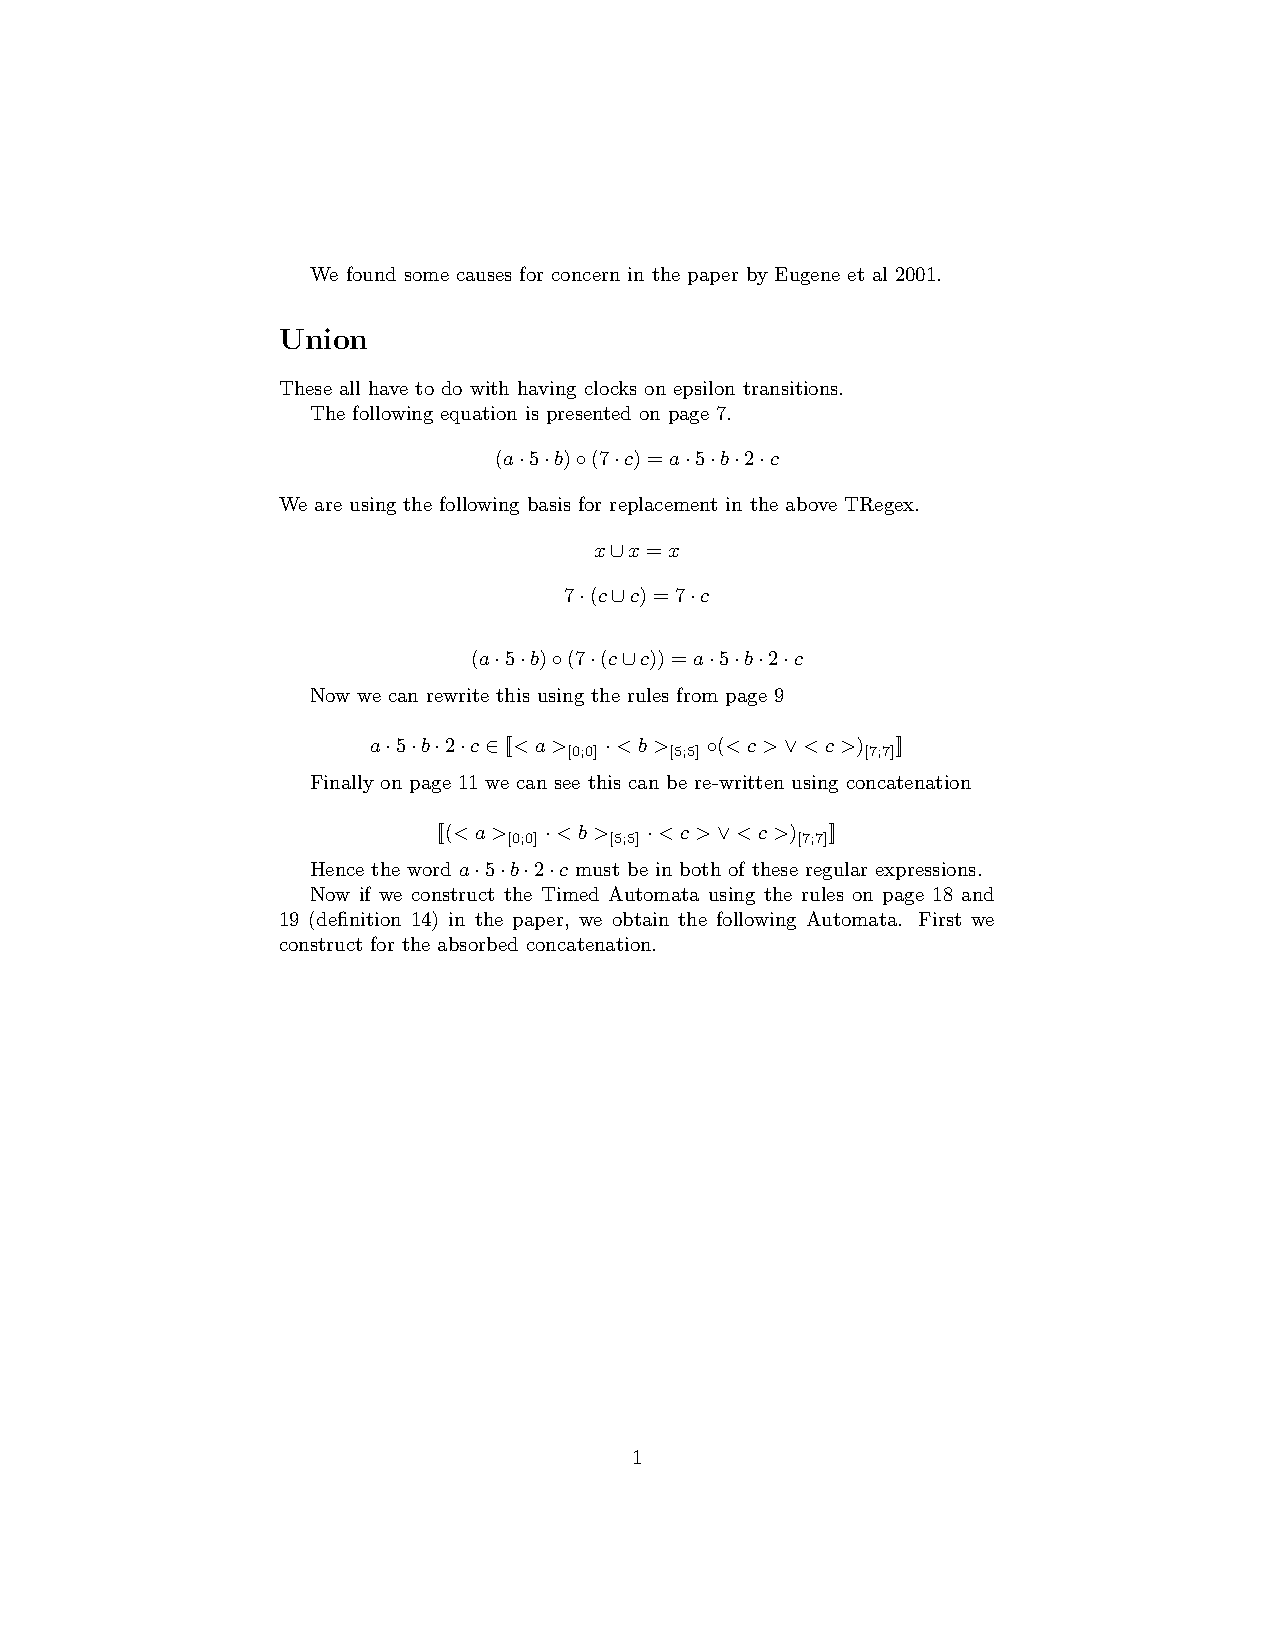
\includepdf[pages=-]{Documents/Appendix/PaperProblems.pdf}

\section{Regular Expressions}\label{sec:RegularExpressions}
\label{app:RegularExpressionTable}
$$p_l=\str{(}$$
$$p_r=\str{)}$$
$$a=\str{+'}$$
$$i=\str{|}$$
$$s=\str{j}$$
$$i_1=\str{j[1;10]}$$
$$i_2=\str{j[1;1]}$$

$$a(n)=p_l^n \circ s \circ (p_r \circ a)^n$$
$$b(n)=p_l^n \circ i_1 \circ (p_r \circ a)^n$$
$$c(n)=i_1^n \circ i \circ i_2$$
$$d(n)=s^n \circ i \circ s$$
$$e(n)=s^n \circ a$$
$$f(n)=(i_2 \circ i)^{n-1} \circ i_2$$

\begin{tabular}{|c|c|}
    \hline
    index & expression \\
    \hline
    0  & a(1) \\
    1  & a(2) \\
    2  & a(4) \\
    \hline
    3  & b(1) \\
    4  & b(2) \\
    5  & b(4) \\
    \hline
    6  & c(64) \\
    7  & c(128) \\
    8  & c(256) \\
    \hline
    9  & d(64) \\
    10 & d(128) \\
    11 & d(256) \\
    \hline
    12 & e(64) \\
    13 & e(128) \\
    14 & e(256) \\
    \hline
    15 & f(1) \\
    16 & f(2) \\
    17 & f(4) \\
    18 & f(8) \\
    19 & f(16) \\
    \hline
\end{tabular}

\section{Benchmark table}\label{sec:BenchmarkTable}
BenchmarkDotNet v0.13.12, EndeavourOS
Intel Core i9-9900K CPU 3.60GHz (Coffee Lake), 1 CPU, 16 logical and 8 physical cores
.NET SDK 8.0.104
  [Host]    : .NET 8.0.4 (8.0.424.16909), X64 RyuJIT AVX2
  MediumRun : .NET 8.0.4 (8.0.424.16909), X64 RyuJIT AVX2
Job=MediumRun  Runtime=.NET 8.0  Toolchain=net8.0  
IterationCount=15  LaunchCount=2  WarmupCount=10  

\begin{sidewaystable}
    \begin{tabular}{|c|c|c|c|c|c|c|c|c|c|}
        \hline
        Method  &   regex   &   Mean                  &   Error             &   StdDev                &   Median                &   Gen0        &   Gen1        &   Gen2        &   Allocated        \\
        \hline
        N       &   0       &   1,634.9 ns            &   9.87 ns           &   14.47 ns              &   1,642.0 ns            &   0.0610      &   0.0000      &   0.0000      &   5.04 KB          \\
        E       &   0       &   2,130.0 ns            &   11.54 ns          &   16.55 ns              &   2,136.5 ns            &   0.0725      &   0.0000      &   0.0000      &   5.98 KB          \\
        S       &   0       &   2,027.1 ns            &   6.68 ns           &   9.14 ns               &   2,028.0 ns            &   0.0687      &   0.0000      &   0.0000      &   5.89 KB          \\
        SS      &   0       &   2,348.2 ns            &   4.18 ns           &   5.86 ns               &   2,348.6 ns            &   0.0801      &   0.0000      &   0.0000      &   6.72 KB          \\
        SE      &   0       &   2,417.8 ns            &   12.02 ns          &   17.62 ns              &   2,408.9 ns            &   0.0801      &   0.0000      &   0.0000      &   6.81 KB          \\
        ES      &   0       &   2,394.1 ns            &   7.05 ns           &   10.33 ns              &   2,397.4 ns            &   0.0801      &   0.0000      &   0.0000      &   6.81 KB          \\
        EE      &   0       &   2,461.5 ns            &   12.50 ns          &   16.25 ns              &   2,459.4 ns            &   0.0839      &   0.0000      &   0.0000      &   6.91 KB          \\
        N       &   1       &   6,036.6 ns            &   56.42 ns          &   82.70 ns              &   6,097.2 ns            &   0.1755      &   0.0000      &   0.0000      &   14.63 KB         \\
        E       &   1       &   8,039.4 ns            &   37.01 ns          &   55.40 ns              &   8,033.7 ns            &   0.2136      &   0.0000      &   0.0000      &   17.63 KB         \\
        S       &   1       &   6,962.4 ns            &   143.05 ns         &   200.54 ns             &   6,799.6 ns            &   0.1907      &   0.0000      &   0.0000      &   15.67 KB         \\
        SS      &   1       &   7,674.8 ns            &   186.12 ns         &   278.58 ns             &   7,669.3 ns            &   0.2060      &   0.0000      &   0.0000      &   17.33 KB         \\
        SE      &   1       &   8,672.8 ns            &   43.27 ns          &   64.77 ns              &   8,675.9 ns            &   0.2289      &   0.0000      &   0.0000      &   19.28 KB         \\
        ES      &   1       &   7,637.9 ns            &   13.79 ns          &   20.21 ns              &   7,645.1 ns            &   0.2136      &   0.0000      &   0.0000      &   17.52 KB         \\
        EE      &   1       &   8,800.2 ns            &   22.93 ns          &   33.62 ns              &   8,798.2 ns            &   0.2289      &   0.0000      &   0.0000      &   19.47 KB         \\
        N       &   2       &   365,861.8 ns          &   1,766.60 ns       &   2,644.17 ns           &   365,384.0 ns          &   7.8125      &   1.9531      &   0.0000      &   668.95 KB        \\
        E       &   2       &   530,259.4 ns          &   7,480.44 ns       &   10,964.74 ns          &   521,403.1 ns          &   11.7188     &   2.9297      &   0.0000      &   971.15 KB        \\
        S       &   2       &   394,797.3 ns          &   576.68 ns          &   863.15 ns             &   394,564.5 ns          &   8.3008      &   2.4414      &   0.0000      &   679.97 KB        \\
        SS      &   2       &   402,027.0 ns          &   936.47 ns          &   1,343.05 ns           &   402,349.1 ns          &   8.3008      &   2.4414      &   0.0000      &   684.61 KB        \\
        SE      &   2       &   533,352.9 ns          &   1,004.86 ns       &   1,472.92 ns           &   533,494.6 ns          &   11.7188     &   2.9297      &   0.0000      &   975.79 KB        \\
        ES      &   2       &   270,858.2 ns          &   1,131.18 ns       &   1,693.10 ns           &   271,188.1 ns          &   6.8359      &   1.4648      &   0.0000      &   566.77 KB        \\
        EE      &   2       &   368,669.7 ns          &   1,670.77 ns       &   2,500.73 ns           &   367,754.5 ns          &   9.2773      &   1.9531      &   0.0000      &   768.92 KB        \\
        N       &   3       &   5,352.0 ns            &   133.94 ns          &   196.33 ns             &   5,504.3 ns            &   0.1526      &   0.0000      &   0.0000      &   12.73 KB         \\
        E       &   3       &   7,892.0 ns            &   40.73 ns           &   55.75 ns              &   7,911.1 ns            &   0.1984      &   0.0000      &   0.0000      &   16.92 KB         \\
        S       &   3       &   6,849.0 ns            &   14.18 ns           &   19.88 ns              &   6,843.2 ns            &   0.1831      &   0.0000      &   0.0000      &   15.16 KB         \\
        SS      &   3       &   5,774.6 ns            &   52.84 ns           &   75.78 ns              &   5,754.8 ns            &   0.1602      &   0.0000      &   0.0000      &   13.2 KB          \\
        SE      &   3       &   6,492.7 ns            &   14.03 ns           &   21.00 ns              &   6,493.8 ns            &   0.1755      &   0.0000      &   0.0000      &   14.71 KB         \\
        ES      &   3       &   6,098.4 ns            &   8.54 ns            &   11.98 ns              &   6,093.4 ns            &   0.1678      &   0.0000      &   0.0000      &   14.21 KB         \\
        EE      &   3       &   6,843.2 ns            &   14.32 ns           &   21.43 ns              &   6,850.9 ns            &   0.1907      &   0.0000      &   0.0000      &   15.73 KB         \\
        N       &   4       &   33,275.6 ns           &   252.37 ns         &   361.95 ns             &   33,037.8 ns           &   0.8545      &   0.0000      &   0.0000      &   69.88 KB         \\
        E       &   4       &   46,225.8 ns           &   59.53 ns          &   89.10 ns              &   46,228.2 ns           &   1.0986      &   0.0610      &   0.0000      &   89.88 KB         \\
        S       &   4       &   39,386.9 ns           &   129.39 ns         &   189.65 ns             &   39,293.8 ns           &   0.9155      &   0.0000      &   0.0000      &   76.1 KB          \\
        SS      &   4       &   18,779.8 ns           &   40.31 ns          &   56.51 ns              &   18,777.7 ns           &   0.4578      &   0.0000      &   0.0000      &   38.41 KB         \\
        SE      &   4       &   21,796.9 ns           &   91.81 ns          &   131.67 ns             &   21,810.0 ns           &   0.5188      &   0.0000      &   0.0000      &   44.69 KB         \\
        ES      &   4       &   17,999.6 ns           &   154.18 ns         &   221.13 ns             &   18,123.7 ns           &   0.4578      &   0.0000      &   0.0000      &   38.64 KB         \\
        EE      &   4       &   20,351.3 ns           &   190.70 ns         &   267.34 ns             &   20,166.2 ns           &   0.5188      &   0.0000      &   0.0000      &   42.84 KB         \\
        N       &   5       &   14,345,441.6 ns       &   106,317.27 ns     &   155,838.48 ns         &   14,360,473.9 ns       &   234.3750    &   218.7500    &   109.3750    &   16675.07 KB      \\
        E       &   5       &   21,889,111.1 ns       &   263,640.17 ns     &   369,586.70 ns         &   21,986,565.8 ns       &   343.7500    &   312.5000    &   125.0000    &   26493.89 KB      \\
        S       &   5       &   15,581,794.2 ns       &   57,071.73 ns      &   85,422.28 ns          &   15,575,622.0 ns       &   234.3750    &   218.7500    &   109.3750    &   17172.08 KB      \\
        SS      &   5       &   6,445,558.3 ns        &   68,269.20 ns      &   102,182.12 ns         &   6,426,665.7 ns        &   93.7500     &   78.1250     &   31.2500     &   7064.14 KB       \\
        SE      &   5       &   9,163,154.7 ns        &   77,369.76 ns      &   115,803.41 ns         &   9,179,374.2 ns        &   140.6250    &   125.0000    &   46.8750     &   11009.93 KB      \\
        ES      &   5       &   3,569,375.9 ns        &   10,572.83 ns      &   15,163.23 ns          &   3,574,975.3 ns        &   58.5938     &   54.6875     &   27.3438     &   4924.5 KB        \\
        EE      &   5       &   5,761,799.7 ns        &   18,151.44 ns      &   24,231.65 ns          &   5,756,398.0 ns        &   101.5625    &   93.7500     &   31.2500     &   7486.67 KB       \\
        \hline
    \end{tabular}
\end{sidewaystable}
\begin{sidewaystable}
    \begin{tabular}{|c|c|c|c|c|c|c|c|c|c|}
        \hline
        Method  &   regex   &   Mean                  &   Error             &   StdDev                &   Median                &   Gen0        &   Gen1        &   Gen2        &   Allocated        \\
        \hline
        N       &   6       &   1,058,482.1 ns        &   4,507.33 ns       &   6,318.65 ns           &   1,055,488.1 ns        &   33.2031     &   13.6719     &   0.0000      &   2774.94 KB       \\
        E       &   6       &   130,202,842.2 ns      &   1,165,246.45 ns   &   1,744,086.02 ns       &   130,263,725.1 ns      &   1750.0000   &   500.0000    &   0.0000      &   158752.09 KB     \\
        S       &   6       &   1,087,341.0 ns        &   4,657.28 ns       &   6,679.32 ns           &   1,086,714.2 ns        &   33.2031     &   13.6719     &   0.0000      &   2799.35 KB       \\
        SS      &   6       &   882,452.6 ns          &   13,988.79 ns      &   19,610.32 ns          &   866,000.2 ns          &   28.3203     &   12.6953     &   0.0000      &   2338.61 KB       \\
        SE      &   6       &   40,407,196.0 ns       &   71,260.18 ns      &   104,452.24 ns         &   40,386,796.0 ns       &   153.8462    &   0.0000      &   0.0000      &   14810.97 KB      \\
        ES      &   6       &   176,619,156.3 ns      &   289,428.88 ns     &   415,090.25 ns         &   176,570,478.8 ns      &   1333.3333   &   333.3333    &   0.0000      &   112051.15 KB     \\
        EE      &   6       &   218,959,171.3 ns      &   546,414.44 ns     &   783,651.26 ns         &   219,103,037.2 ns      &   1333.3333   &   333.3333    &   0.0000      &   124523.45 KB     \\
        N       &   7       &   3,484,513.8 ns        &   29,916.06 ns      &   44,776.95 ns          &   3,486,315.8 ns        &   117.1875    &   113.2813    &   0.0000      &   9617.03 KB       \\
        E       &   7       &   1,547,147,583.4 ns    &   8,026,410.82 ns   &   11,765,008.91 ns      &   1,549,048,615.0 ns    &   15000.0000  &   1000.0000   &   0.0000      &   1245220.51 KB    \\
        S       &   7       &   3,566,171.7 ns        &   13,619.88 ns      &   19,963.84 ns          &   3,574,351.7 ns        &   117.1875    &   89.8438     &   0.0000      &   9667.24 KB       \\
        SS      &   7       &   3,037,890.7 ns        &   4,994.25 ns       &   7,475.16 ns           &   3,036,768.7 ns        &   105.4688    &   82.0313     &   0.0000      &   8618.71 KB       \\
        SE      &   7       &   548,214,611.6 ns      &   3,979,121.03 ns   &   5,955,761.00 ns       &   548,884,287.0 ns      &   1000.0000   &   0.0000      &   0.0000      &   102171.73 KB     \\
        ES      &   7       &   2,454,885,536.6 ns    &   4,488,862.38 ns   &   6,579,716.27 ns       &   2,454,092,008.0 ns    &   10000.0000  &   1000.0000   &   0.0000      &   884427.52 KB     \\
        EE      &   7       &   2,995,173,650.1 ns    &   18,242,043.28 ns  &   25,572,796.96 ns      &   3,012,707,120.0 ns    &   11000.0000  &   1000.0000   &   0.0000      &   977979.83 KB     \\
        N       &   8       &   12,697,373.2 ns       &   21,288.66 ns      &   29,843.72 ns          &   12,697,516.0 ns       &   437.5000    &   421.8750    &   0.0000      &   36055.38 KB      \\
        E       &   8       &   21,617,377,726.5 ns   &   288,524,813.91 ns &   431,850,356.17 ns     &   21,785,903,112.0 ns   &   120000.0000 &   3000.0000   &   1000.0000   &   9871874.21 KB    \\
        S       &   8       &   12,737,119.2 ns       &   118,281.48 ns     &   177,038.15 ns         &   12,737,861.9 ns       &   437.5000    &   421.8750    &   0.0000      &   36160.29 KB      \\
        SS      &   8       &   11,038,197.9 ns       &   124,283.70 ns     &   178,243.96 ns         &   11,168,117.2 ns       &   390.6250    &   375.0000    &   0.0000      &   33125.43 KB      \\
        SE      &   8       &   8,368,043,360.9 ns    &   48,410,361.58 ns  &   72,458,349.80 ns      &   8,392,358,432.5 ns    &   9000.0000   &   1000.0000   &   0.0000      &   756806.44 KB     \\
        ES      &   8       &   34,743,709,646.1 ns   &   671,871,810.11 ns &   963,578,473.62 ns     &   33,914,698,636.5 ns   &   86000.0000  &   4000.0000   &   1000.0000   &   7031719.82 KB    \\
        EE      &   8       &   42,989,588,867.6 ns   &   984,507,838.03 ns &   1,473,564,976.07 ns   &   42,965,379,610.5 ns   &   94000.0000  &   5000.0000   &   1000.0000   &   7755400.13 KB    \\
        N       &   9       &   466,234.1 ns          &   3,325.83 ns       &   4,977.94 ns           &   466,314.1 ns          &   17.0898     &   3.9063      &   0.0000      &   1433.59 KB       \\
        E       &   9       &   498,700.1 ns          &   2,530.69 ns       &   3,547.67 ns           &   496,592.0 ns          &   17.5781     &   3.9063      &   0.0000      &   1450.21 KB       \\
        S       &   9       &   495,040.8 ns          &   1,200.99 ns       &   1,797.58 ns           &   494,859.9 ns          &   17.5781     &   2.9297      &   0.0000      &   1449.53 KB       \\
        SS      &   9       &   480,547.2 ns          &   2,326.44 ns       &   3,482.11 ns           &   480,458.0 ns          &   17.0898     &   3.4180      &   0.0000      &   1412.54 KB       \\
        SE      &   9       &   479,276.2 ns          &   2,269.46 ns       &   3,326.54 ns           &   477,245.7 ns          &   17.0898     &   3.4180      &   0.0000      &   1413.22 KB       \\
        ES      &   9       &   488,593.6 ns          &   1,034.18 ns       &   1,483.18 ns           &   488,766.5 ns          &   16.6016     &   3.9063      &   0.0000      &   1419.92 KB       \\
        EE      &   9       &   485,500.6 ns          &   1,923.13 ns       &   2,818.90 ns           &   486,744.9 ns          &   17.0898     &   3.4180      &   0.0000      &   1420.59 KB       \\
        N       &   10      &   1,552,189.8 ns        &   4,112.69 ns       &   6,155.67 ns           &   1,552,457.7 ns        &   58.5938     &   21.4844     &   0.0000      &   4915.88 KB       \\
        E       &   10      &   1,640,849.7 ns        &   8,326.43 ns       &   12,204.78 ns          &   1,648,903.8 ns        &   60.5469     &   19.5313     &   0.0000      &   4948.77 KB       \\
        S       &   10      &   1,614,288.9 ns        &   11,917.71 ns      &   17,468.83 ns          &   1,622,644.2 ns        &   60.5469     &   13.6719     &   0.0000      &   4948.09 KB       \\
        SS      &   10      &   1,572,649.2 ns        &   10,392.10 ns      &   15,554.41 ns          &   1,572,842.8 ns        &   58.5938     &   19.5313     &   0.0000      &   4872.73 KB       \\
        SE      &   10      &   1,567,464.8 ns        &   2,522.52 ns       &   3,697.48 ns           &   1,567,685.0 ns        &   58.5938     &   21.4844     &   0.0000      &   4873.41 KB       \\
        ES      &   10      &   1,613,948.4 ns        &   3,672.80 ns       &   5,497.28 ns           &   1,612,299.2 ns        &   58.5938     &   17.5781     &   0.0000      &   4887.9 KB        \\
        EE      &   10      &   1,609,730.6 ns        &   9,676.92 ns       &   13,878.34 ns          &   1,608,487.3 ns        &   58.5938     &   19.5313     &   0.0000      &   4888.58 KB       \\
        N       &   11      &   5,441,492.3 ns        &   28,112.35 ns      &   42,077.25 ns          &   5,443,850.1 ns        &   210.9375    &   125.0000    &   0.0000      &   17662.75 KB      \\
        E       &   11      &   5,715,852.7 ns        &   6,080.15 ns       &   8,523.52 ns           &   5,714,072.2 ns        &   210.9375    &   117.1875    &   0.0000      &   17730.58 KB      \\
        S       &   11      &   5,623,561.5 ns        &   15,302.34 ns      &   22,429.97 ns          &   5,620,045.6 ns        &   210.9375    &   117.1875    &   0.0000      &   17729.9 KB       \\
        SS      &   11      &   5,609,644.0 ns        &   11,036.86 ns      &   15,472.14 ns          &   5,608,025.8 ns        &   210.9375    &   109.3750    &   0.0000      &   17579.53 KB      \\
        SE      &   11      &   5,491,159.6 ns        &   23,273.37 ns      &   34,113.80 ns          &   5,488,853.9 ns        &   210.9375    &   125.0000    &   0.0000      &   17580.21 KB      \\
        ES      &   11      &   5,510,257.2 ns        &   10,030.97 ns      &   14,703.27 ns          &   5,509,956.2 ns        &   210.9375    &   101.5625    &   0.0000      &   17611.64 KB      \\
        EE      &   11      &   5,583,399.1 ns        &   38,305.29 ns      &   56,147.39 ns          &   5,545,160.0 ns        &   210.9375    &   109.3750    &   0.0000      &   17612.32 KB      \\
        \hline
    \end{tabular}
\end{sidewaystable}
\begin{sidewaystable}
    \begin{tabular}{|c|c|c|c|c|c|c|c|c|c|}
        \hline
        Method  &   regex   &   Mean                  &   Error             &   StdDev                &   Median                &   Gen0        &   Gen1        &   Gen2        &   Allocated        \\
        \hline
        N       &   12      &   438,380.5 ns          &   1,855.76 ns       &   2,661.48 ns           &   439,950.3 ns          &   16.1133     &   3.4180      &   0.0000      &   1344.23 KB       \\
        E       &   12      &   455,207.0 ns          &   2,573.48 ns       &   3,851.86 ns           &   455,383.9 ns          &   16.6016     &   3.9063      &   0.0000      &   1365.41 KB       \\
        S       &   12      &   454,085.5 ns          &   1,587.65 ns       &   2,225.66 ns           &   452,693.8 ns          &   16.6016     &   3.9063      &   0.0000      &   1358.13 KB       \\
        SS      &   12      &   446,637.5 ns          &   2,502.28 ns       &   3,507.85 ns           &   448,952.7 ns          &   16.6016     &   3.9063      &   0.0000      &   1358.96 KB       \\
        SE      &   12      &   459,558.8 ns          &   3,345.14 ns       &   4,797.50 ns           &   460,456.6 ns          &   16.6016     &   3.9063      &   0.0000      &   1366.24 KB       \\
        ES      &   12      &   450,664.2 ns          &   4,110.95 ns       &   5,762.97 ns           &   453,953.1 ns          &   16.6016     &   3.4180      &   0.0000      &   1359.05 KB       \\
        EE      &   12      &   458,164.2 ns          &   1,655.20 ns       &   2,426.17 ns           &   459,618.3 ns          &   16.6016     &   3.4180      &   0.0000      &   1366.34 KB       \\
        N       &   13      &   1,477,177.5 ns        &   1,462.66 ns       &   2,050.45 ns           &   1,477,241.6 ns        &   56.6406     &   23.4375     &   0.0000      &   4732.96 KB       \\
        E       &   13      &   1,511,804.0 ns        &   6,297.65 ns       &   8,828.43 ns           &   1,510,737.8 ns        &   56.6406     &   23.4375     &   0.0000      &   4777.54 KB       \\
        S       &   13      &   1,501,376.8 ns        &   2,245.42 ns       &   3,291.30 ns           &   1,501,064.8 ns        &   56.6406     &   25.3906     &   0.0000      &   4762.46 KB       \\
        SS      &   13      &   1,530,411.6 ns        &   7,332.51 ns       &   10,516.06 ns          &   1,529,417.4 ns        &   56.6406     &   23.4375     &   0.0000      &   4763.29 KB       \\
        SE      &   13      &   1,525,024.1 ns        &   1,776.38 ns       &   2,547.63 ns           &   1,525,165.1 ns        &   56.6406     &   23.4375     &   0.0000      &   4778.37 KB       \\
        ES      &   13      &   1,521,473.5 ns        &   2,837.26 ns       &   4,158.81 ns           &   1,522,342.5 ns        &   56.6406     &   25.3906     &   0.0000      &   4763.38 KB       \\
        EE      &   13      &   1,532,103.4 ns        &   5,675.10 ns       &   7,955.70 ns           &   1,536,225.3 ns        &   56.6406     &   23.4375     &   0.0000      &   4778.46 KB       \\
        N       &   14      &   5,328,251.7 ns        &   9,635.87 ns       &   13,508.14 ns          &   5,329,462.9 ns        &   210.9375    &   140.6250    &   0.0000      &   17289.26 KB      \\
        E       &   14      &   5,406,084.6 ns        &   19,226.40 ns      &   27,573.93 ns          &   5,406,630.6 ns        &   210.9375    &   140.6250    &   0.0000      &   17384.65 KB      \\
        S       &   14      &   5,323,808.2 ns        &   44,007.39 ns      &   64,505.45 ns          &   5,367,876.2 ns        &   210.9375    &   140.6250    &   0.0000      &   17352.64 KB      \\
        SS      &   14      &   5,503,721.2 ns        &   6,996.40 ns       &   10,034.03 ns          &   5,504,045.1 ns        &   210.9375    &   132.8125    &   0.0000      &   17353.47 KB      \\
        SE      &   14      &   5,348,640.0 ns        &   43,266.43 ns      &   62,051.42 ns          &   5,388,433.8 ns        &   210.9375    &   132.8125    &   0.0000      &   17385.48 KB      \\
        ES      &   14      &   5,359,476.8 ns        &   18,235.38 ns      &   24,960.80 ns          &   5,371,932.9 ns        &   210.9375    &   117.1875    &   0.0000      &   17353.56 KB      \\
        EE      &   14      &   5,515,236.7 ns        &   13,930.15 ns      &   20,418.63 ns          &   5,513,582.8 ns        &   210.9375    &   125.0000    &   0.0000      &   17385.58 KB      \\
        N       &   15      &   625.1 ns              &   2.92 ns           &   4.09 ns               &   624.9 ns              &   0.0286      &   0.0000      &   0.0000      &   2.38 KB          \\
        E       &   15      &   1,512.2 ns            &   3.56 ns           &   5.33 ns               &   1,511.6 ns            &   0.0572      &   0.0000      &   0.0000      &   4.75 KB          \\
        S       &   15      &   1,117.2 ns            &   3.44 ns           &   5.04 ns               &   1,117.0 ns            &   0.0439      &   0.0000      &   0.0000      &   3.73 KB          \\
        SS      &   15      &   1,125.3 ns            &   5.79 ns           &   8.66 ns               &   1,128.6 ns            &   0.0439      &   0.0000      &   0.0000      &   3.73 KB          \\
        SE      &   15      &   1,511.3 ns            &   2.95 ns           &   4.41 ns               &   1,511.1 ns            &   0.0572      &   0.0000      &   0.0000      &   4.75 KB          \\
        ES      &   15      &   1,130.7 ns            &   2.07 ns           &   3.09 ns               &   1,130.8 ns            &   0.0439      &   0.0000      &   0.0000      &   3.73 KB          \\
        EE      &   15      &   1,507.7 ns            &   3.85 ns           &   5.76 ns               &   1,507.3 ns            &   0.0572      &   0.0000      &   0.0000      &   4.75 KB          \\
        N       &   16      &   4,363.0 ns            &   7.50 ns           &   11.00 ns              &   4,362.4 ns            &   0.1450      &   0.0000      &   0.0000      &   12.3 KB          \\
        E       &   16      &   6,262.7 ns            &   11.33 ns          &   16.25 ns              &   6,264.8 ns            &   0.1831      &   0.0000      &   0.0000      &   15.5 KB          \\
        S       &   16      &   5,341.5 ns            &   12.86 ns          &   18.03 ns              &   5,339.1 ns            &   0.1678      &   0.0000      &   0.0000      &   13.86 KB         \\
        SS      &   16      &   4,758.7 ns            &   42.89 ns          &   64.20 ns              &   4,750.0 ns            &   0.1602      &   0.0000      &   0.0000      &   13.37 KB         \\
        SE      &   16      &   5,500.0 ns            &   35.59 ns          &   53.27 ns              &   5,500.8 ns            &   0.1755      &   0.0000      &   0.0000      &   14.63 KB         \\
        ES      &   16      &   5,522.4 ns            &   43.80 ns          &   62.82 ns              &   5,477.6 ns            &   0.1831      &   0.0000      &   0.0000      &   15.4 KB          \\
        EE      &   16      &   6,226.0 ns            &   83.36 ns          &   122.19 ns             &   6,319.5 ns            &   0.1984      &   0.0000      &   0.0000      &   16.66 KB         \\
        N       &   17      &   23,745.2 ns           &   49.79 ns          &   74.52 ns              &   23,749.4 ns           &   0.7019      &   0.0305      &   0.0000      &   59.38 KB         \\
        E       &   17      &   34,755.7 ns           &   254.33 ns         &   364.76 ns             &   34,751.1 ns           &   0.9766      &   0.0000      &   0.0000      &   83.24 KB         \\
        S       &   17      &   26,400.8 ns           &   37.83 ns          &   55.46 ns              &   26,394.5 ns           &   0.7324      &   0.0305      &   0.0000      &   62.1 KB          \\
        SS      &   17      &   12,385.5 ns           &   80.16 ns          &   117.49 ns             &   12,404.3 ns           &   0.3967      &   0.0000      &   0.0000      &   33.36 KB         \\
        SE      &   17      &   13,643.0 ns           &   72.74 ns          &   108.87 ns             &   13,646.4 ns           &   0.4272      &   0.0000      &   0.0000      &   36.13 KB         \\
        ES      &   17      &   15,279.1 ns           &   166.63 ns         &   238.98 ns             &   15,109.0 ns           &   0.4578      &   0.0000      &   0.0000      &   39.59 KB         \\
        EE      &   17      &   15,860.8 ns           &   102.35 ns         &   146.79 ns             &   15,930.8 ns           &   0.4883      &   0.0000      &   0.0000      &   40.86 KB         \\
        \hline
    \end{tabular}
\end{sidewaystable}
\begin{sidewaystable}
    \begin{tabular}{|c|c|c|c|c|c|c|c|c|c|}
        \hline
        Method  &   regex   &   Mean                  &   Error             &   StdDev                &   Median                &   Gen0        &   Gen1        &   Gen2        &   Allocated        \\
        \hline
        N       &   18      &   404,847.5 ns          &   2,978.33 ns       &   4,457.83 ns           &   404,539.6 ns          &   11.2305     &   1.9531      &   0.0000      &   917.55 KB        \\
        E       &   18      &   1,039,886.9 ns        &   2,864.49 ns       &   4,198.73 ns           &   1,041,291.5 ns        &   29.2969     &   13.6719     &   0.0000      &   2515.32 KB       \\
        S       &   18      &   441,169.9 ns          &   1,979.55 ns       &   2,839.01 ns           &   442,855.6 ns          &   11.2305     &   4.3945      &   0.0000      &   934.43 KB        \\
        SS      &   18      &   29,107.9 ns           &   100.08 ns         &   146.70 ns             &   29,081.2 ns           &   0.9155      &   0.0305      &   0.0000      &   76.75 KB         \\
        SE      &   18      &   33,642.9 ns           &   89.41 ns          &   128.23 ns             &   33,611.3 ns           &   1.0376      &   0.0000      &   0.0000      &   86.02 KB         \\
        ES      &   18      &   35,954.9 ns           &   194.75 ns         &  279.30 ns              &   35,966.1 ns           &   1.0376      &   0.0000      &   0.0000      &   89.39 KB         \\
        EE      &   18      &   36,579.7 ns           &   63.92 ns          &   93.69 ns              &   36,585.2 ns           &   1.0986      &   0.0000      &   0.0000      &   90.66 KB         \\
        N       &   19      &   388,956,329.8 ns      &   25,239,927.44 ns  &   37,777,934.96 ns      &   396,098,198.0 ns      &   6000.0000   &   6000.0000   &   4000.0000   &   315469.2 KB      \\
        E       &   19      &   2,007,281,088.0 ns    &   63,324,812.08 ns  &   90,818,553.26 ns      &   2,036,489,152.5 ns    &   27000.0000  &   9000.0000   &   5000.0000   &   1955655.8 KB     \\
        S       &   19      &   439,493,172.0 ns      &   25,717,693.35 ns  &   36,883,547.32 ns      &   449,660,552.0 ns      &   6000.0000   &   6000.0000   &   4000.0000   &   321366.52 KB     \\
        SS      &   19      &   69,831.3 ns           &   180.95 ns           &   270.84 ns             &   69,889.2 ns           &   2.0752      &   0.1221      &   0.0000      &   174.71 KB        \\
        SE      &   19      &   85,871.9 ns           &   412.77 ns           &   591.99 ns             &   85,651.6 ns           &   2.4414      &   0.1221      &   0.0000      &   208.98 KB        \\
        ES      &   19      &   85,025.0 ns           &   159.55 ns           &   233.87 ns             &   85,044.3 ns           &   2.3193      &   0.1221      &   0.0000      &   193.98 KB        \\
        EE      &   19      &   87,248.7 ns           &   784.32 ns           &   1,149.64 ns           &   87,974.0 ns           &   2.3193      &   0.1221      &   0.0000      &   195.24 KB        \\
        \hline    
    \end{tabular}
\end{sidewaystable}

\section{Benchmark graphs}\label{sec:BenchmarkGraphs}
\subsection{0-2}
\resizebox{\textwidth}{!}{
    % 0,1,2
\plot{1,2,4}
{(1,1634.9)(2,6036.6)(4,365861.8)}
{(1,2130.0)(2,8039.4)(4,530259.4)}
{(1,2027.1)(2,6962.4)(4,394797.3)}
{(1,2348.2)(2,7674.8)(4,402027)}
{(1,2417.8)(2,8672.8)(4,533352.9)}
{(1,2394.1)(2,7637.9)(4,270858.2)}
{(1,2461.5)(2,8800.2)(4,368669.7)}
    % 0,1,2
\plot{1,2,4}
{(1,1634.9)(2,6036.6)(4,365861.8)}
{(1,2130.0)(2,8039.4)(4,530259.4)}
{(1,2027.1)(2,6962.4)(4,394797.3)}
{(1,2348.2)(2,7674.8)(4,402027)}
{(1,2417.8)(2,8672.8)(4,533352.9)}
{(1,2394.1)(2,7637.9)(4,270858.2)}
{(1,2461.5)(2,8800.2)(4,368669.7)}
}
\subsection{3-5}
\resizebox{\textwidth}{!}{
    % 3,4,5
\plot{1,2,4}
{(1,5352.0)(2,33275.6)(4,14345441.6)}
{(1,7892.0)(2,46225.8)(4,21889111.1)}
{(1,6849.0)(2,39386.9)(4,15581794.2)}
{(1,5774.6)(2,18779.8)(4,6445558.3)}
{(1,6492.7)(2,21796.9)(4,9163154.7)}
{(1,6098.4)(2,17999.6)(4,3569375.9)}
{(1,6843.2)(2,20351.3)(4,5761799.7)}
    % 3,4,5
\plot{1,2,4}
{(1,5352.0)(2,33275.6)(4,14345441.6)}
{(1,7892.0)(2,46225.8)(4,21889111.1)}
{(1,6849.0)(2,39386.9)(4,15581794.2)}
{(1,5774.6)(2,18779.8)(4,6445558.3)}
{(1,6492.7)(2,21796.9)(4,9163154.7)}
{(1,6098.4)(2,17999.6)(4,3569375.9)}
{(1,6843.2)(2,20351.3)(4,5761799.7)}
}
\subsection{6-8}
\resizebox{\textwidth}{!}{
    % 6,7,8
\plotmem{64,128,256}
{(64,2774.94)    (128,9617.03)     (256,36055.38)}
{(64,158752.09)  (128,1245220.51)  (256,9871874.21)}
{(64,2799.35)    (128,9667.24)     (256,36160.29)}
{(64,2338.61)    (128,8618.71)     (256,33125.43)}
{(64,14810.97)   (128,102171.73)  (256,756806.44)}
{(64,112051.15)  (128,884427.52)  (256,7031719.82)}
{(64,124523.45)  (128,977979.83)  (256,7755400.13)}
    % 6,7,8
\plotmem{64,128,256}
{(64,2774.94)    (128,9617.03)     (256,36055.38)}
{(64,158752.09)  (128,1245220.51)  (256,9871874.21)}
{(64,2799.35)    (128,9667.24)     (256,36160.29)}
{(64,2338.61)    (128,8618.71)     (256,33125.43)}
{(64,14810.97)   (128,102171.73)  (256,756806.44)}
{(64,112051.15)  (128,884427.52)  (256,7031719.82)}
{(64,124523.45)  (128,977979.83)  (256,7755400.13)}
}
\subsection{9-11}
\resizebox{\textwidth}{!}{
    % 9,10,11
\plotmem{64,128,256}
{(64,1433.59)(128,4915.88)(256,17662.75)}
{(64,1450.21)(128,4948.77)(256,17730.58)}
{(64,1449.53)(128,4948.09)(256,17729.9)}
{(64,1412.54)(128,4872.73)(256,17579.53)}
{(64,1413.22)(128,4873.41)(256,17580.21)}
{(64,1419.92)(128,4887.9)(256,17611.64)}
{(64,1420.59)(128,4888.58)(256,17612.32)}
    % 9,10,11
\plotmem{64,128,256}
{(64,1433.59)(128,4915.88)(256,17662.75)}
{(64,1450.21)(128,4948.77)(256,17730.58)}
{(64,1449.53)(128,4948.09)(256,17729.9)}
{(64,1412.54)(128,4872.73)(256,17579.53)}
{(64,1413.22)(128,4873.41)(256,17580.21)}
{(64,1419.92)(128,4887.9)(256,17611.64)}
{(64,1420.59)(128,4888.58)(256,17612.32)}
}
\subsection{12-14}
\resizebox{\textwidth}{!}{
    % 12,13,14
\plotmem{64,128,256}
{(64,1344.23)(128,4732.96)(256,17289.26)}
{(64,1365.41)(128,4777.54)(256,17384.65)}
{(64,1358.13)(128,4762.46)(256,17352.64)}
{(64,1358.96)(128,4763.29)(256,17353.47)}
{(64,1366.24)(128,4778.37)(256,17385.48)}
{(64,1359.05)(128,4763.38)(256,17353.56)}
{(64,1366.34)(128,4778.46)(256,17385.58)}
    % 12,13,14
\plotmem{64,128,256}
{(64,1344.23)(128,4732.96)(256,17289.26)}
{(64,1365.41)(128,4777.54)(256,17384.65)}
{(64,1358.13)(128,4762.46)(256,17352.64)}
{(64,1358.96)(128,4763.29)(256,17353.47)}
{(64,1366.24)(128,4778.37)(256,17385.48)}
{(64,1359.05)(128,4763.38)(256,17353.56)}
{(64,1366.34)(128,4778.46)(256,17385.58)}
}
\subsection{15-19}
\resizebox{\textwidth}{!}{
    % 15,16,17,18,19
\plotmem{1,2,4,8,16}
{(1,2.38) (2,12.3)(4,59.38)(8,917.55)   (16,315469.2)}
{(1,4.75)(2,15.5)(4,83.24)(8,2515.32)  (16,1955655.8)}
{(1,3.73)(2,13.86)(4,62.1)(8,934.43)   (16,321366.52)}
{(1,3.73)(2,13.37)(4,33.36)(8,76.75)    (16,174.71)}
{(1,4.75)(2,14.63)(4,36.13)(8,86.02)    (16,208.98)}
{(1,3.73)(2,15.4)(4,39.59)(8,89.39)    (16,193.98)}
{(1,4.75)(2,16.66)(4,40.86)(8,90.66)    (16,195.24)}
    % 15,16,17,18,19
\plotmem{1,2,4,8,16}
{(1,2.38) (2,12.3)(4,59.38)(8,917.55)   (16,315469.2)}
{(1,4.75)(2,15.5)(4,83.24)(8,2515.32)  (16,1955655.8)}
{(1,3.73)(2,13.86)(4,62.1)(8,934.43)   (16,321366.52)}
{(1,3.73)(2,13.37)(4,33.36)(8,76.75)    (16,174.71)}
{(1,4.75)(2,14.63)(4,36.13)(8,86.02)    (16,208.98)}
{(1,3.73)(2,15.4)(4,39.59)(8,89.39)    (16,193.98)}
{(1,4.75)(2,16.66)(4,40.86)(8,90.66)    (16,195.24)}
}
\end{document}
